\section{BÖLÜM: SİSTEM MİMARİSİ VE YÖNTEM}
\label{bolum3}

Bu bölümde model roket uçuş bilgisayarı için tasarlanan yazılımsal ve donanımsal mimarinin detayları sunulmaktadır. Sistemin katmanlı yapısı, donanım birimlerinin kullanımı ve FreeRTOS eksenindeki görev mimarisi açıklanmıştır.

\subsection{Katmanlı Yazılım Mimarisi}
\label{katmanli_yazilim_mimarisi}

Model roketin aviyonik yazılım sistemi, modülerliğin sağlanması ve donanım bağımlılığının en aza indirilmesi amacıyla 4 temel katmandan (Donanım, HAL, Sürücü/Middleware, Uygulama) oluşacak şekilde tasarlanmıştır. Her katman yalnızca kendi altındaki katmanlar ile iletişim kuracak şekilde (tek yönlü bağımlılık ilkesi) yapılandırılmıştır.

\begin{itemize}
    \item \textbf{Donanım Katmanı (Hardware):} STM32F446 mikrodenetleyicisi, sensörler (BMI088, BME280, L86) ve iletişim yolları (I2C, SPI, USART).
    \item \textbf{HAL Katmanı (Hardware Abstraction Layer):} STMicroelectronics tarafından sağlanan ve STM32CubeMX ile otomatik üretilen bu katman, donanım kayıtçılarının (register) doğrudan manipüle edilmesi yerine standart API'ler sunar. Uçuş güvenilirliği için CubeMX tarafından \textit{Core/Src/} altında oluşturulan `gpio.c`, `i2c.c` gibi başlatma kodlarına dışarıdan müdahale edilmemiş, tüm işlevsellik kullanıcı dosyalarında gerçeklenmiştir.
    \item \textbf{Sürücü/Middleware Katmanı:} FreeRTOS işletim sistemi çekirdeği ile birlikte sensörlerin (BME280, BMI088 vb.) spesifik konfigürasyonlarını içeren sürücü dosyalarını barındırır.
    \item \textbf{Uygulama Katmanı (Application):} Uçuş algoritmalarının, sensör füzyonunun (Mahony, Kalman) ve tepe noktası tayini gibi uçuş fazlarını idare eden operasyonel görevlerin (Tasks) bulunduğu en üst katmandır.
\end{itemize}

\begin{figure}[H]
    \centering
    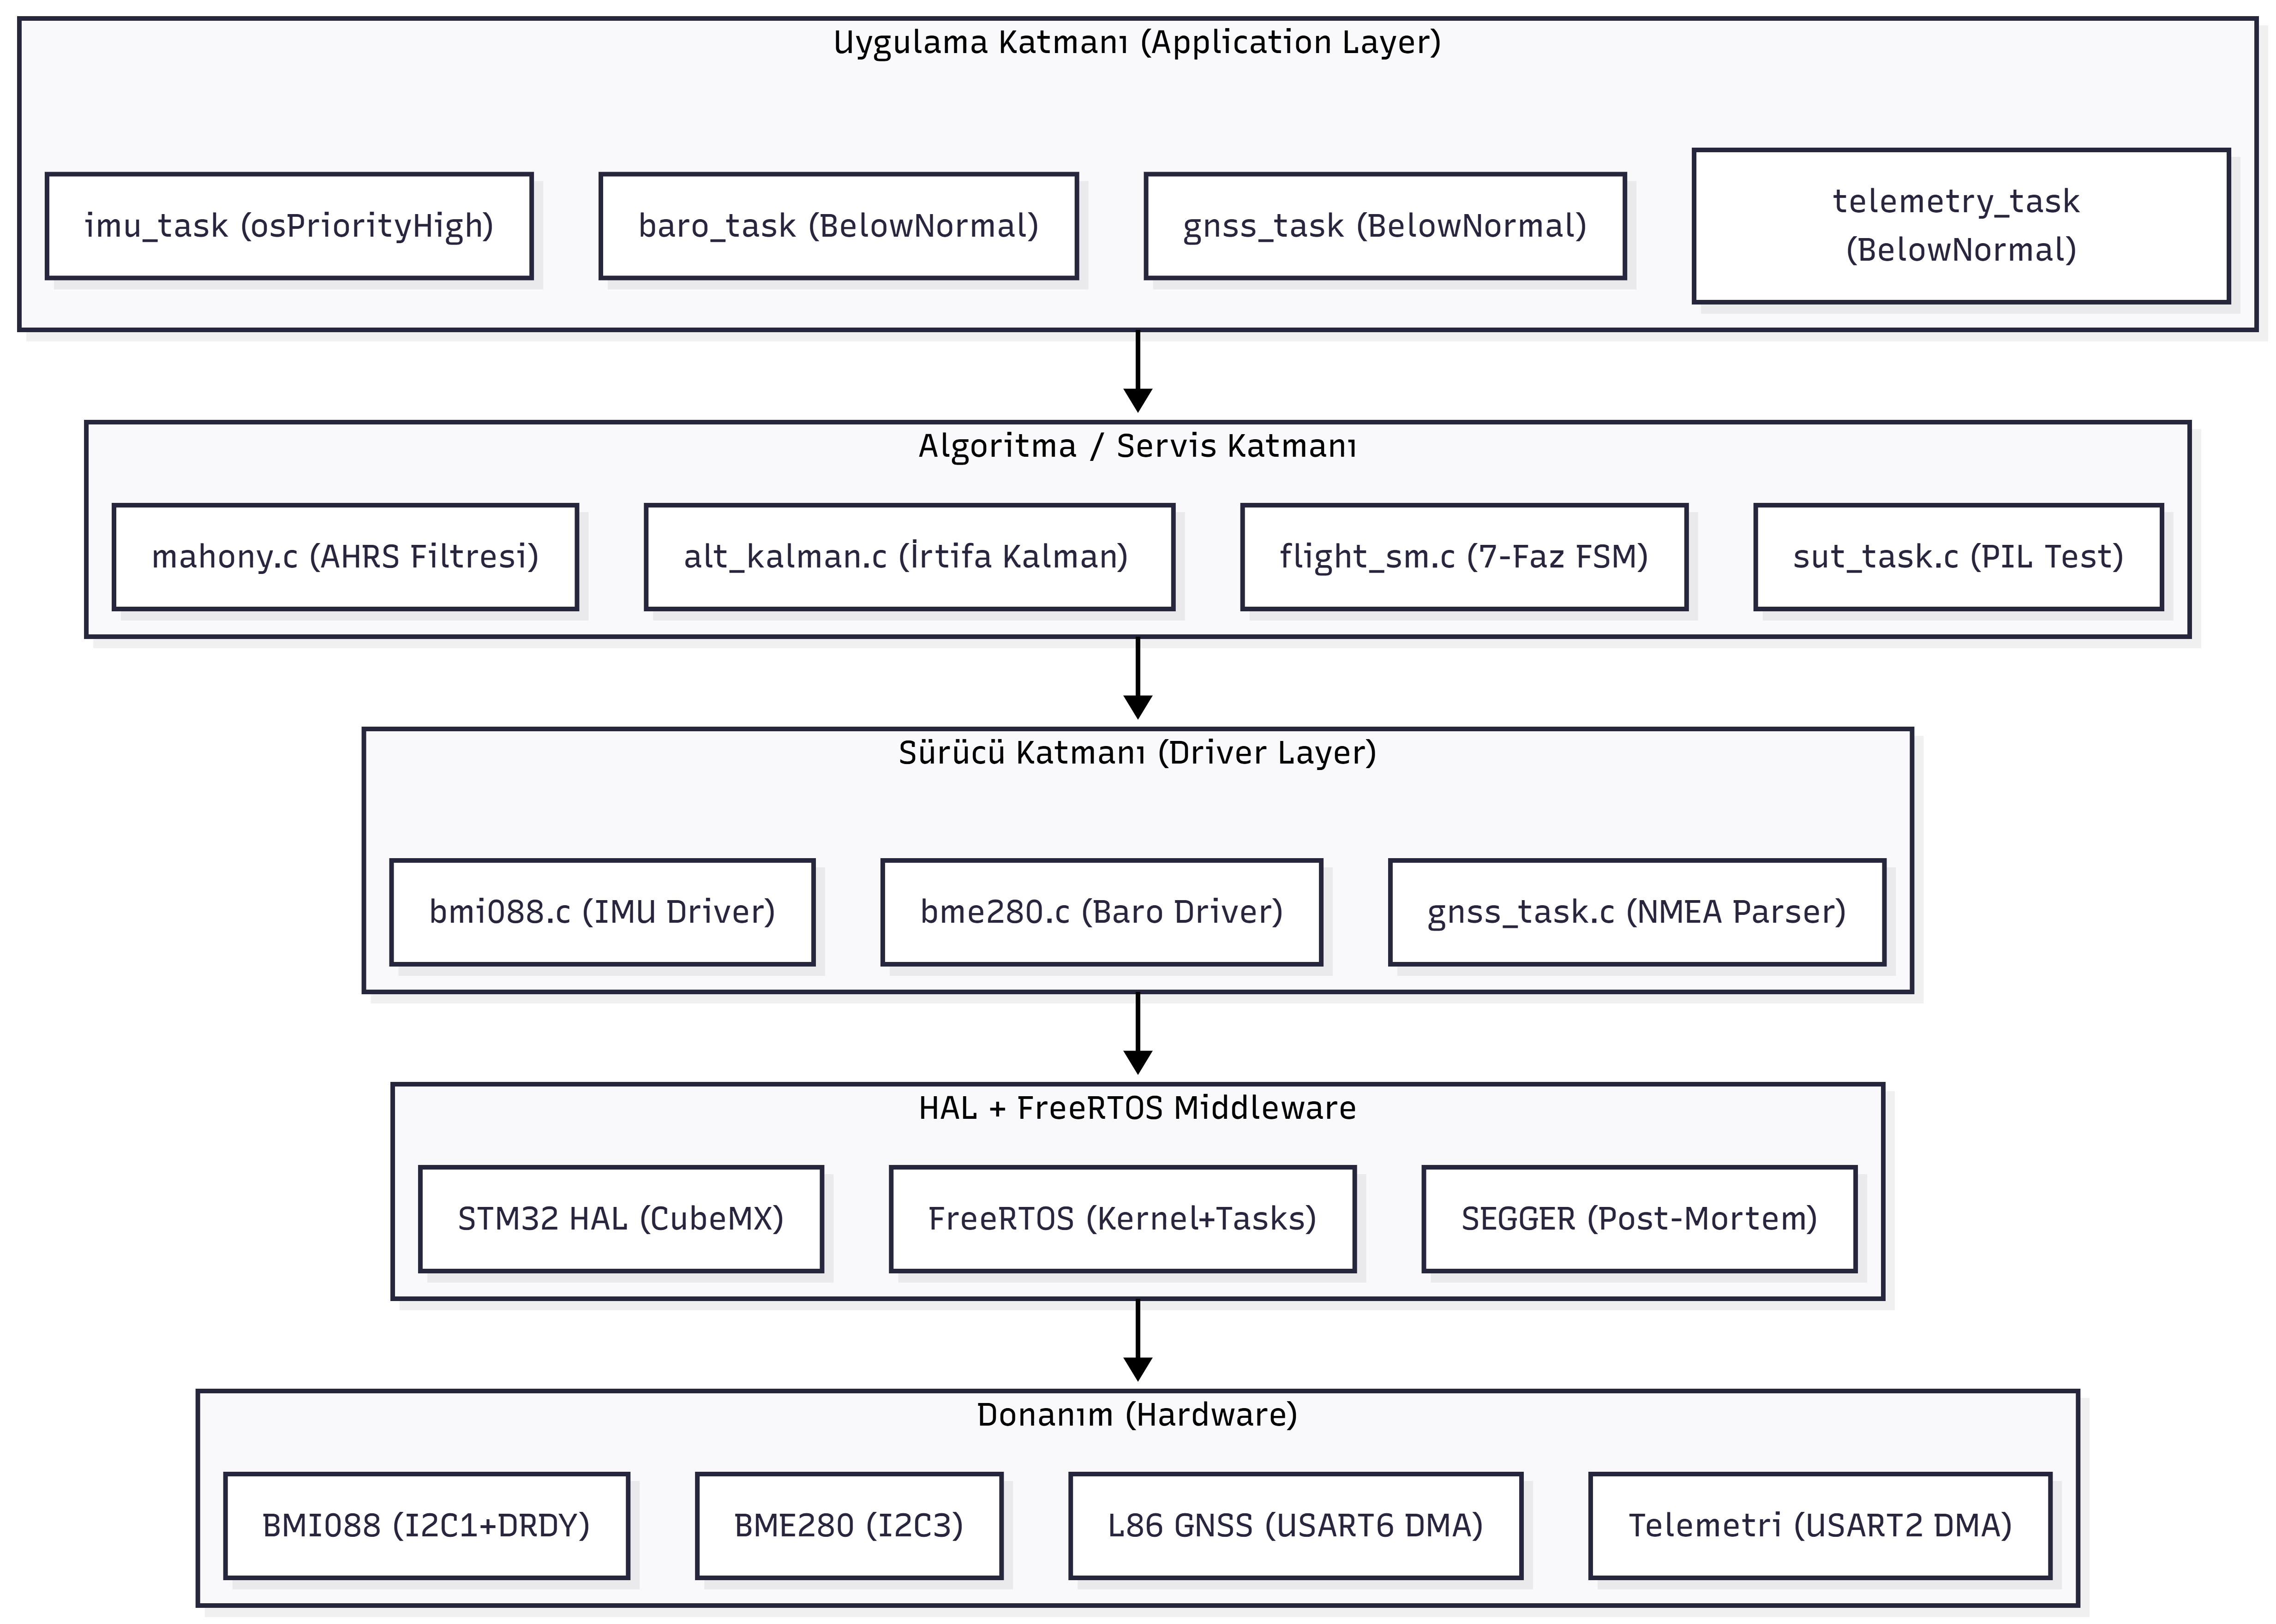
\includegraphics[width=0.8\textwidth]{sekiller/KatmanlıYazılımMimarisi(4 katman).png}
    \caption{Uçuş Bilgisayarı 4 Katmanlı Yazılım Mimarisi ve SIT/SUT Entegrasyonu}
    \label{fig:katmanli_mimari}
\end{figure}

\subsection{Donanım Haritası ve Çevresel Birimler}
\label{donanim_haritasi}

Uçuş algoritmasının ihtiyaç duyduğu verilerin toplanabilmesi için mikrodenetleyicinin çevresel birimleri spesifik görevlere atanmıştır. Haberleşme birimlerinde işlemciyi (CPU) meşgul etmemek adına Doğrudan Bellek Erişimi (DMA) mimarisi uygulanmıştır. BME280 sensörü I2C3, BMI088 (İvmeölçer ve Jiroskop) ise I2C1 veri yolları üzerinden sisteme bağlanmıştır. Ayrıca veri hazır kesmesini asenkron olarak tetiklemek için EXTI (Dış Kesme) hatları kullanılmıştır.

Sistemin, elektromanyetik parazitler veya olası bir yazılımsal döngü tıkanıklığı (deadlock) karşısında kilitlenmemesi adına Donanımsal Bağımsız Zamanlayıcı (IWDG - Independent Watchdog) kurulmuştur. IWDG yapılandırmasında frekans bölücü (prescaler) değeri 256, yeniden yükleme (reload) değeri ise 249 olarak atanmış olup yaklaşık 2 saniyelik bir \textit{timeout} (zaman aşımı) süresi sağlanmıştır. Belirtilen bu süre içinde barometre görevi Watchdog'u beslemezse (yenilemezse), donanım otomatik olarak sistem sıfırlaması (reset) uygular.

\begin{table}[htbp]
    \centering
    \caption{Donanım Haritası ve Çevresel Birim Görevleri}
    \label{tab:donanim_haritasi}
    \begin{tabular}{|l|l|l|l|}
    \hline
    \textbf{Çevresel Birim} & \textbf{Pin Ataması} & \textbf{Protokol} & \textbf{Sorumlu Görev / Modül} \\ \hline
    I2C1 & PB8 (SCL), PB9 (SDA) & I2C (Hızlı Mod) & BMI088 (İvme \& Jiroskop) \\ \hline
    I2C3 & PA8 (SCL), PC9 (SDA) & I2C (Standart Mod) & BME280 (Barometre) \\ \hline
    EXTI3 & PB3 & GPIO Kesmesi & BMI088 İvme DRDY Sinyali \\ \hline
    EXTI4 & PB4 & GPIO Kesmesi & BMI088 Jiroskop DRDY Sinyali \\ \hline
    USART6 & DMA RX & Seri Haberleşme & GNSS (L86) Modülü \\ \hline
    USART2 & DMA TX/RX & Seri Haberleşme & Telemetri (SIT / ST-Link VCP) \\ \hline
    IWDG & Dahili (LSI) & - & Donanımsal Hata Koruması \\ \hline
    BUZZER & PB14 & GPIO & Durum ve Uyarı Sinyali \\ \hline
    \end{tabular}
\end{table}

\subsection{FreeRTOS Görev Mimarisi}
\label{freertos_gorev_mimarisi}

Operasyonel kısıtlar doğrultusunda FreeRTOS mimarisi üzerinde birbirini kesebilen ve durum önceliklerine göre sıralanmış toplam dört yapısal görev (Task) tasarlanmıştır. SUT (System Under Test) modunda donanımsal sensör okuması yapılmadığından, IMU, Baro, GNSS ve Telemetri görevleri \verb|vTaskDelay| ile uyku döngülerinde tutularak \textit{sut\_task} modülüne alan açmaktadır.

Gerçek donanım modunda; ISR'dan başlayan sensör tetiklemeleri bir zincirleme aksiyon üretir. Bu deterministik akış: DRDY (Data Ready) Pin $\rightarrow$ EXTI ISR $\rightarrow$ \verb|xTaskNotifyFromISR| $\rightarrow$ IMU görevi uyanması $\rightarrow$ DMA transferini başlatması $\rightarrow$ Tamamlanma (DMA Complete) Kesmesi $\rightarrow$ Parse işlemi $\rightarrow$ Snapshot Güncellemesi şeklinde işletilir.

Snapshot mekanizması, görevlerin \textit{veriye tek kaynaklı dönüşümünü} garanti altına almak için Derinliği 1 (\textit{depth=1}) boyutunda olan FreeRTOS kuyruklarıyla inşa edilmiştir. Yığın (Stack) bellek taşmalarına karşı FreeRTOS konfigürasyonunda \verb|configCHECK_FOR_STACK_OVERFLOW| seviyesi 2'ye çekilmiştir.

\begin{table}[htbp]
    \centering
    \caption{FreeRTOS Görev Öncelikleri ve Temel Özellikleri}
    \label{tab:gorev_tablosu}
    \begin{tabular}{|l|l|p{1.5cm}|p{3.5cm}|p{3cm}|}
    \hline
    \textbf{Görev Adı} & \textbf{Öncelik} & \textbf{Stack (Byte)} & \textbf{Tetikleyici} & \textbf{İşlem / Periyot} \\ \hline
    imu\_task & osPriorityHigh & $512 \times 4$ & Donanım Kesmesi & Mahony, Snapshot \\ \hline
    baro\_task & osPriorityBelowNormal & $512 \times 4$ & 100 ms Periyot & Kalman, Flight SM \\ \hline
    gnss\_task & osPriorityBelowNormal & $512 \times 4$ & DMA Circular RX & 1 Hz NMEA Parse \\ \hline
    telemetry\_task & osPriorityBelowNormal & $256 \times 4$ & İletişim Hazır & 50 Hz UART Gönderimi \\ \hline
    \end{tabular}
\end{table}

Aşağıdaki kod parçasında, ivme veya jiroskop kesmelerinden (\textit{notify}) uyanan IMU görevinin DMA işlem zincirini (StateMachine) yönetmesi gösterilmektedir:

\begin{lstlisting}[language=C, caption={IMU Görevi İçerisindeki DMA Durum Makinesi Yönetimi}]
if (dma_state == DMA_IDLE) {
    if (acc_pending) {
        if (bmi088_start_accel_dma(k_bmi_cfg.hi2c, s_acc_buf) == HAL_OK) {
            dma_state   = DMA_READING_ACC;
            acc_pending = false;
        }
    } else if (gyro_pending) {
        if (bmi088_start_gyro_dma(k_bmi_cfg.hi2c, s_gyro_buf) == HAL_OK) {
            dma_state    = DMA_READING_GYRO;
            gyro_pending = false;
        }
    }
}
\end{lstlisting}

\subsection{Sensör Sürücüleri}
\label{sensor_suruculeri}

\subsubsection{BMI088 IMU Sürücüsü (I2C + DMA + DRDY IRQ)}
Veri toplama mimarisinin temeli olan BMI088 İvmeölçer ve Jiroskop sensörü, mimari yapısı gereği sistemde hız kısıtı oluşturmaması için iki ayrı donanım adresi halinde ele alınmıştır. İlgili veri okuma süreci tamamıyla kesme tabanlı asenkron bir yöntemle sağlanmaktadır:

\begin{itemize}
    \item \textbf{DRDY (Data Ready) Pin Tetiklemesi:} Her iki sensörden gelen (İvme EXTI3, Jiroskop EXTI4) veri hazır pinleri donanımsal kesme (Interrupt) fonksiyonunu tetikler.
    \item \textbf{DMA Non-blocking Okuma:} \verb|bmi088_start_accel_dma| fonksiyonu kullanılarak işlemci işgal edilmeden veriler bellek adreslerine çekilir.
    \item \textbf{Anlamlı Veriye (Parse) Dönüştürme:} $\pm 12g$ olarak alınan ivme aralığı \verb|bmi088_parse_accel| komutu ile $m/s^2$'ye çevrilir; 2000 dps aralığındaki jiroskop verisi rad/s birimine dönüştürülür.
\end{itemize}

\begin{figure}[H]
    \centering
    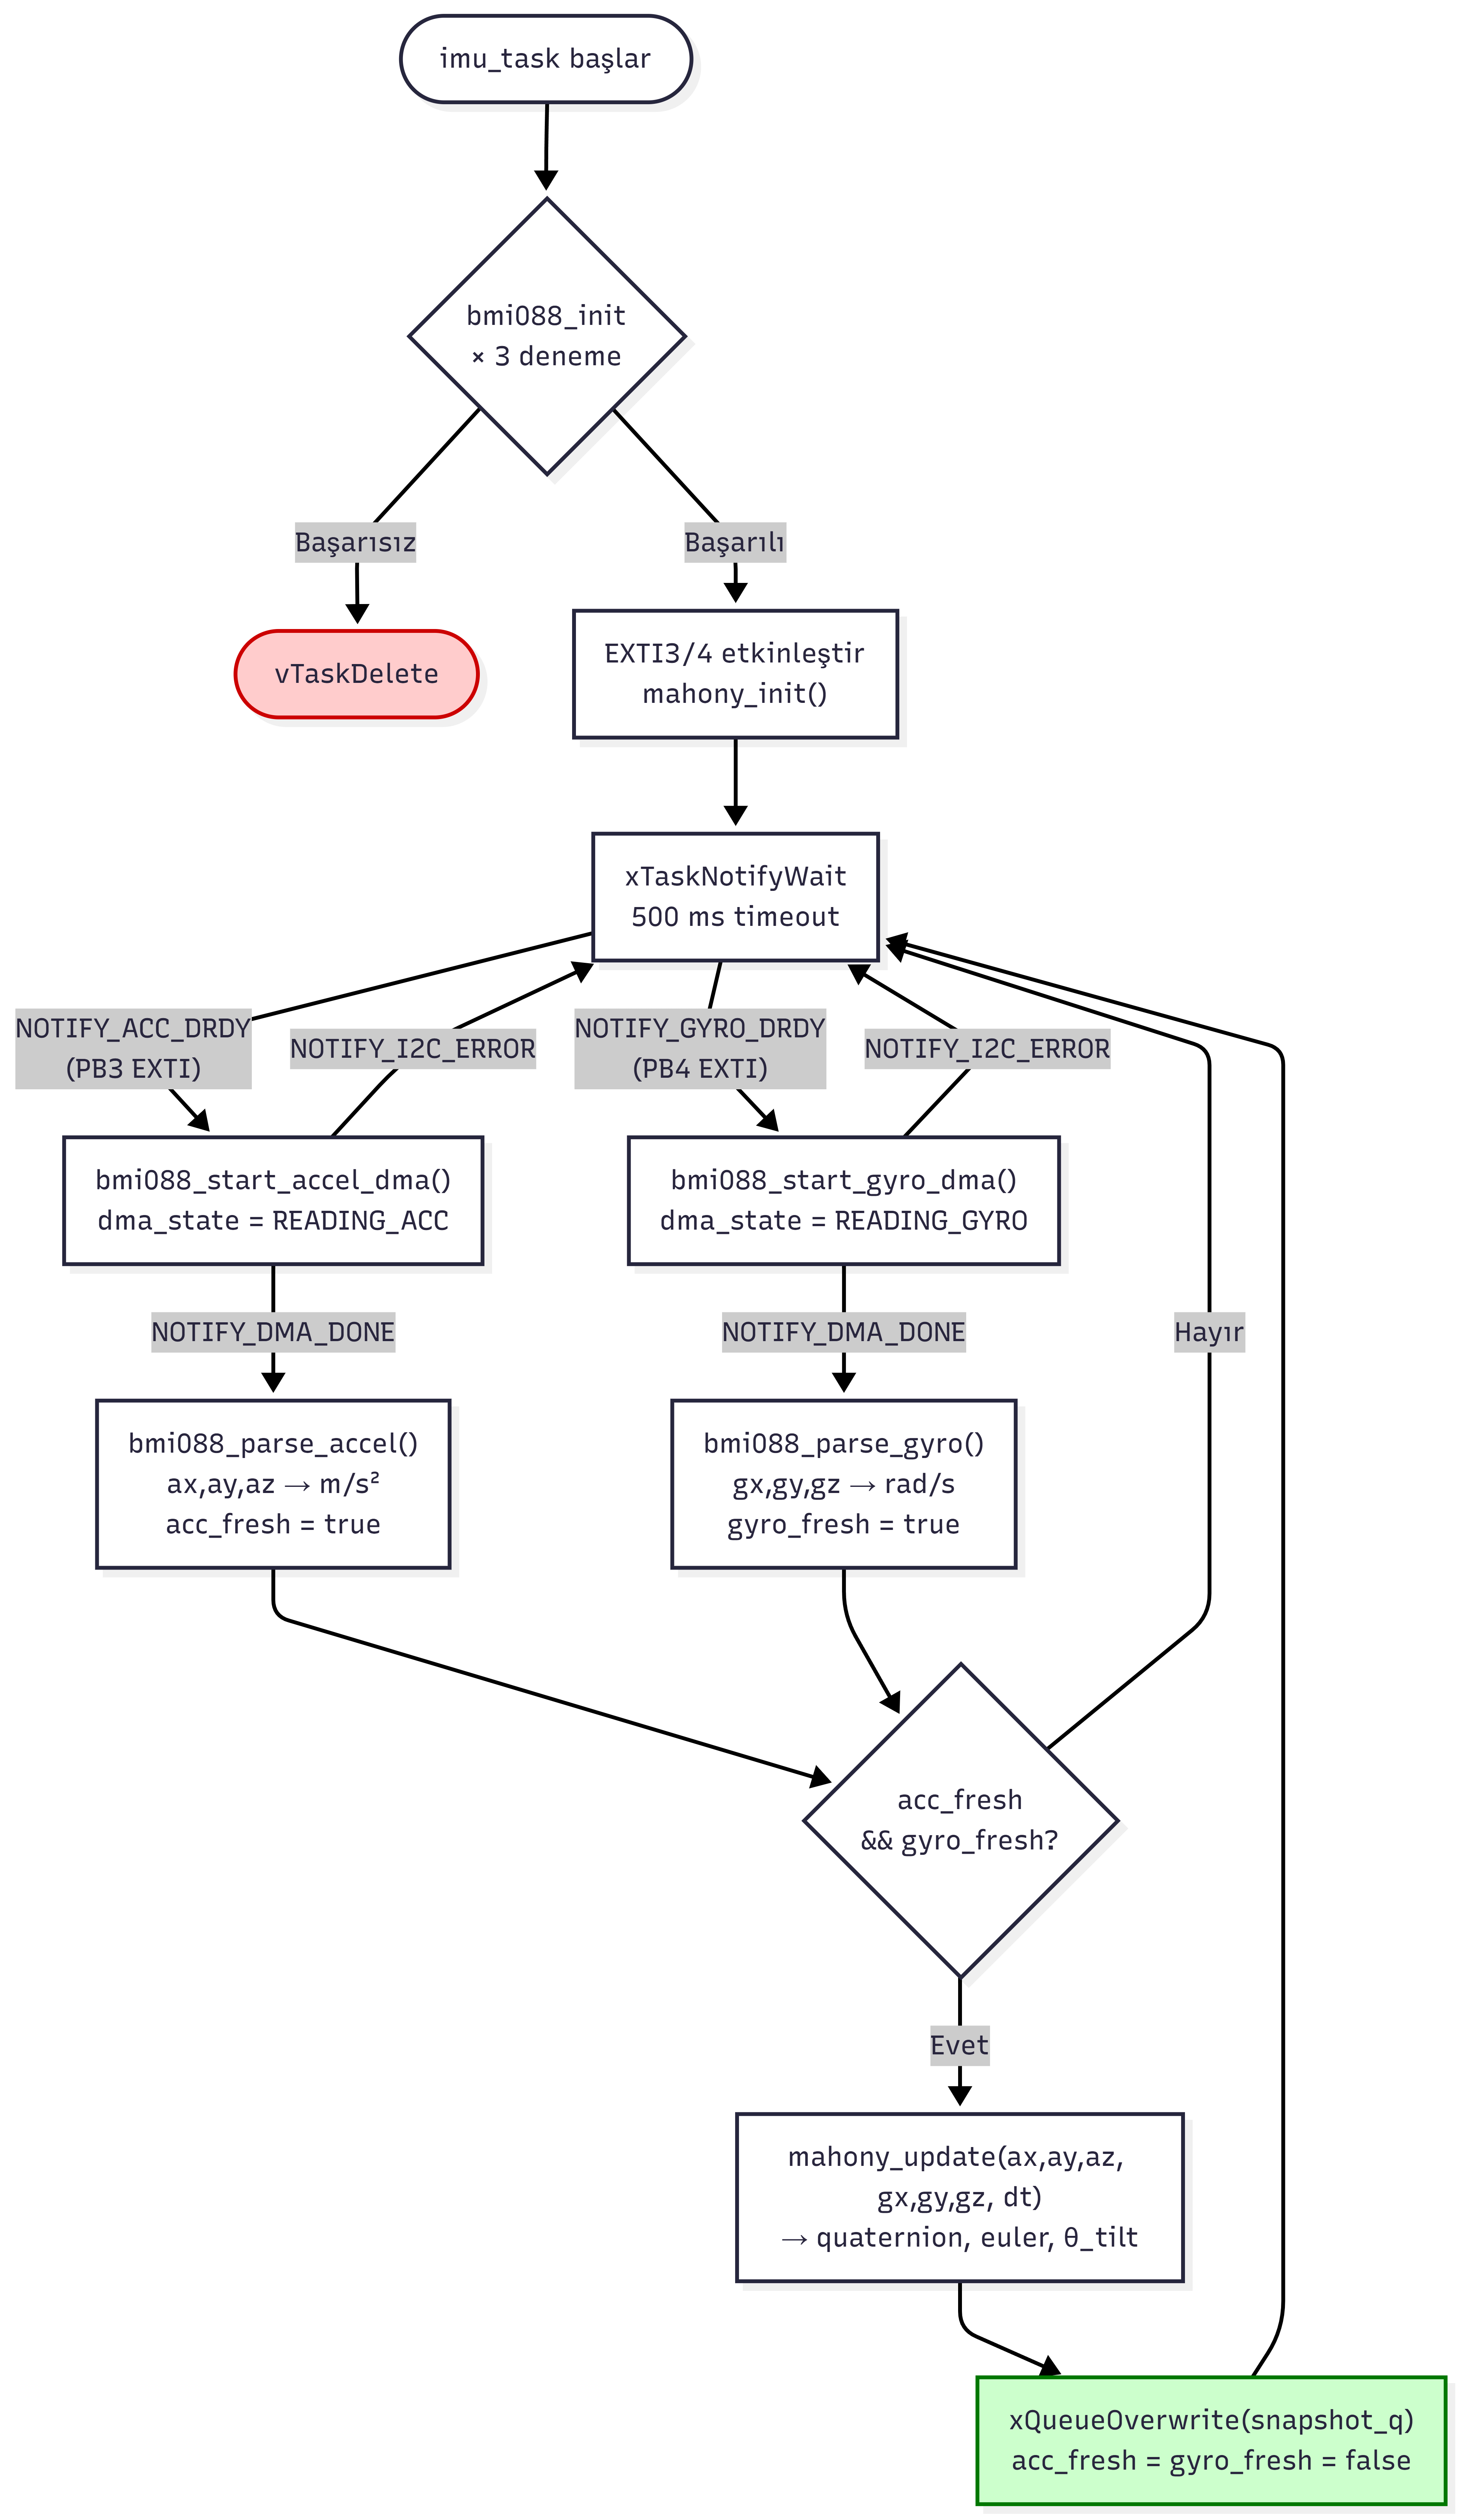
\includegraphics[width=\textwidth]{sekiller/IMU_Pipeline.png}
    \caption{BMI088 IMU Veri İşleme Hattı (Pipeline) ve Mahony Entegrasyonu}
    \label{fig:imu_pipeline}
\end{figure}

Başlangıç aşamasında meydana gelebilecek iletişim hatalarına karşı 3 denemeli bir tekrar (\textit{retry}) döngüsü kurgulanmıştır. Başarısızlık durumunda yazılım baro-only (sadece barometre) modunda çalışmaya devam etmek üzere ilgili görevi FreeRTOS üzerinden siler.

\begin{lstlisting}[language=C, caption={BMI088 İletişim Başlangıç ve Retry Döngüsü (\texttt{imu\_task.c})}]
int retries = 3;
while (bmi088_init(&k_bmi_cfg) != 0) {
    if (--retries == 0) {
        vTaskDelete(NULL); // Sensor yok, gorevi sil
        return;
    }
    HAL_I2C_DeInit(&hi2c1);
    __HAL_RCC_I2C1_FORCE_RESET();
    vTaskDelay(pdMS_TO_TICKS(10));
    __HAL_RCC_I2C1_RELEASE_RESET();
    vTaskDelay(pdMS_TO_TICKS(10));
    MX_I2C1_Init();
    vTaskDelay(pdMS_TO_TICKS(30));
}
\end{lstlisting}

\subsubsection{BME280 Barometrik Basınç Sürücüsü}
Sistemdeki barometrik basınç verisi I2C3 yolu üzerinden saniyede 10 örnek (10 Hz) alınacak şekilde tasarlanmıştır. \verb|vTaskDelayUntil| fonksiyonu kullanılarak, görevin her koşulda 100 ms periyot kısıtına uyması (\textit{catch-up}) güvence altına alınmıştır. 

Sensör üzerinden ham olarak alınan basınç ve sıcaklık verisi Bosch datasheet katsayılarına göre kompanze edilip irtifaya çevrilmektedir. İrtifa referans kalibrasyonu (boot evresinde alınan ilk değer) referans noktası kabul edilerek roketin yerden yüksekliği saptanır. Görev sonrasında ise sırasıyla \verb|alt_kalman_update| tetiklenerek hız-ivme kestirimi tamamlanır ve \verb|flight_sm_update| adımına girilir. Barometre döngüsünün ekseni şu şekildedir:

\begin{figure}[H]
    \centering
    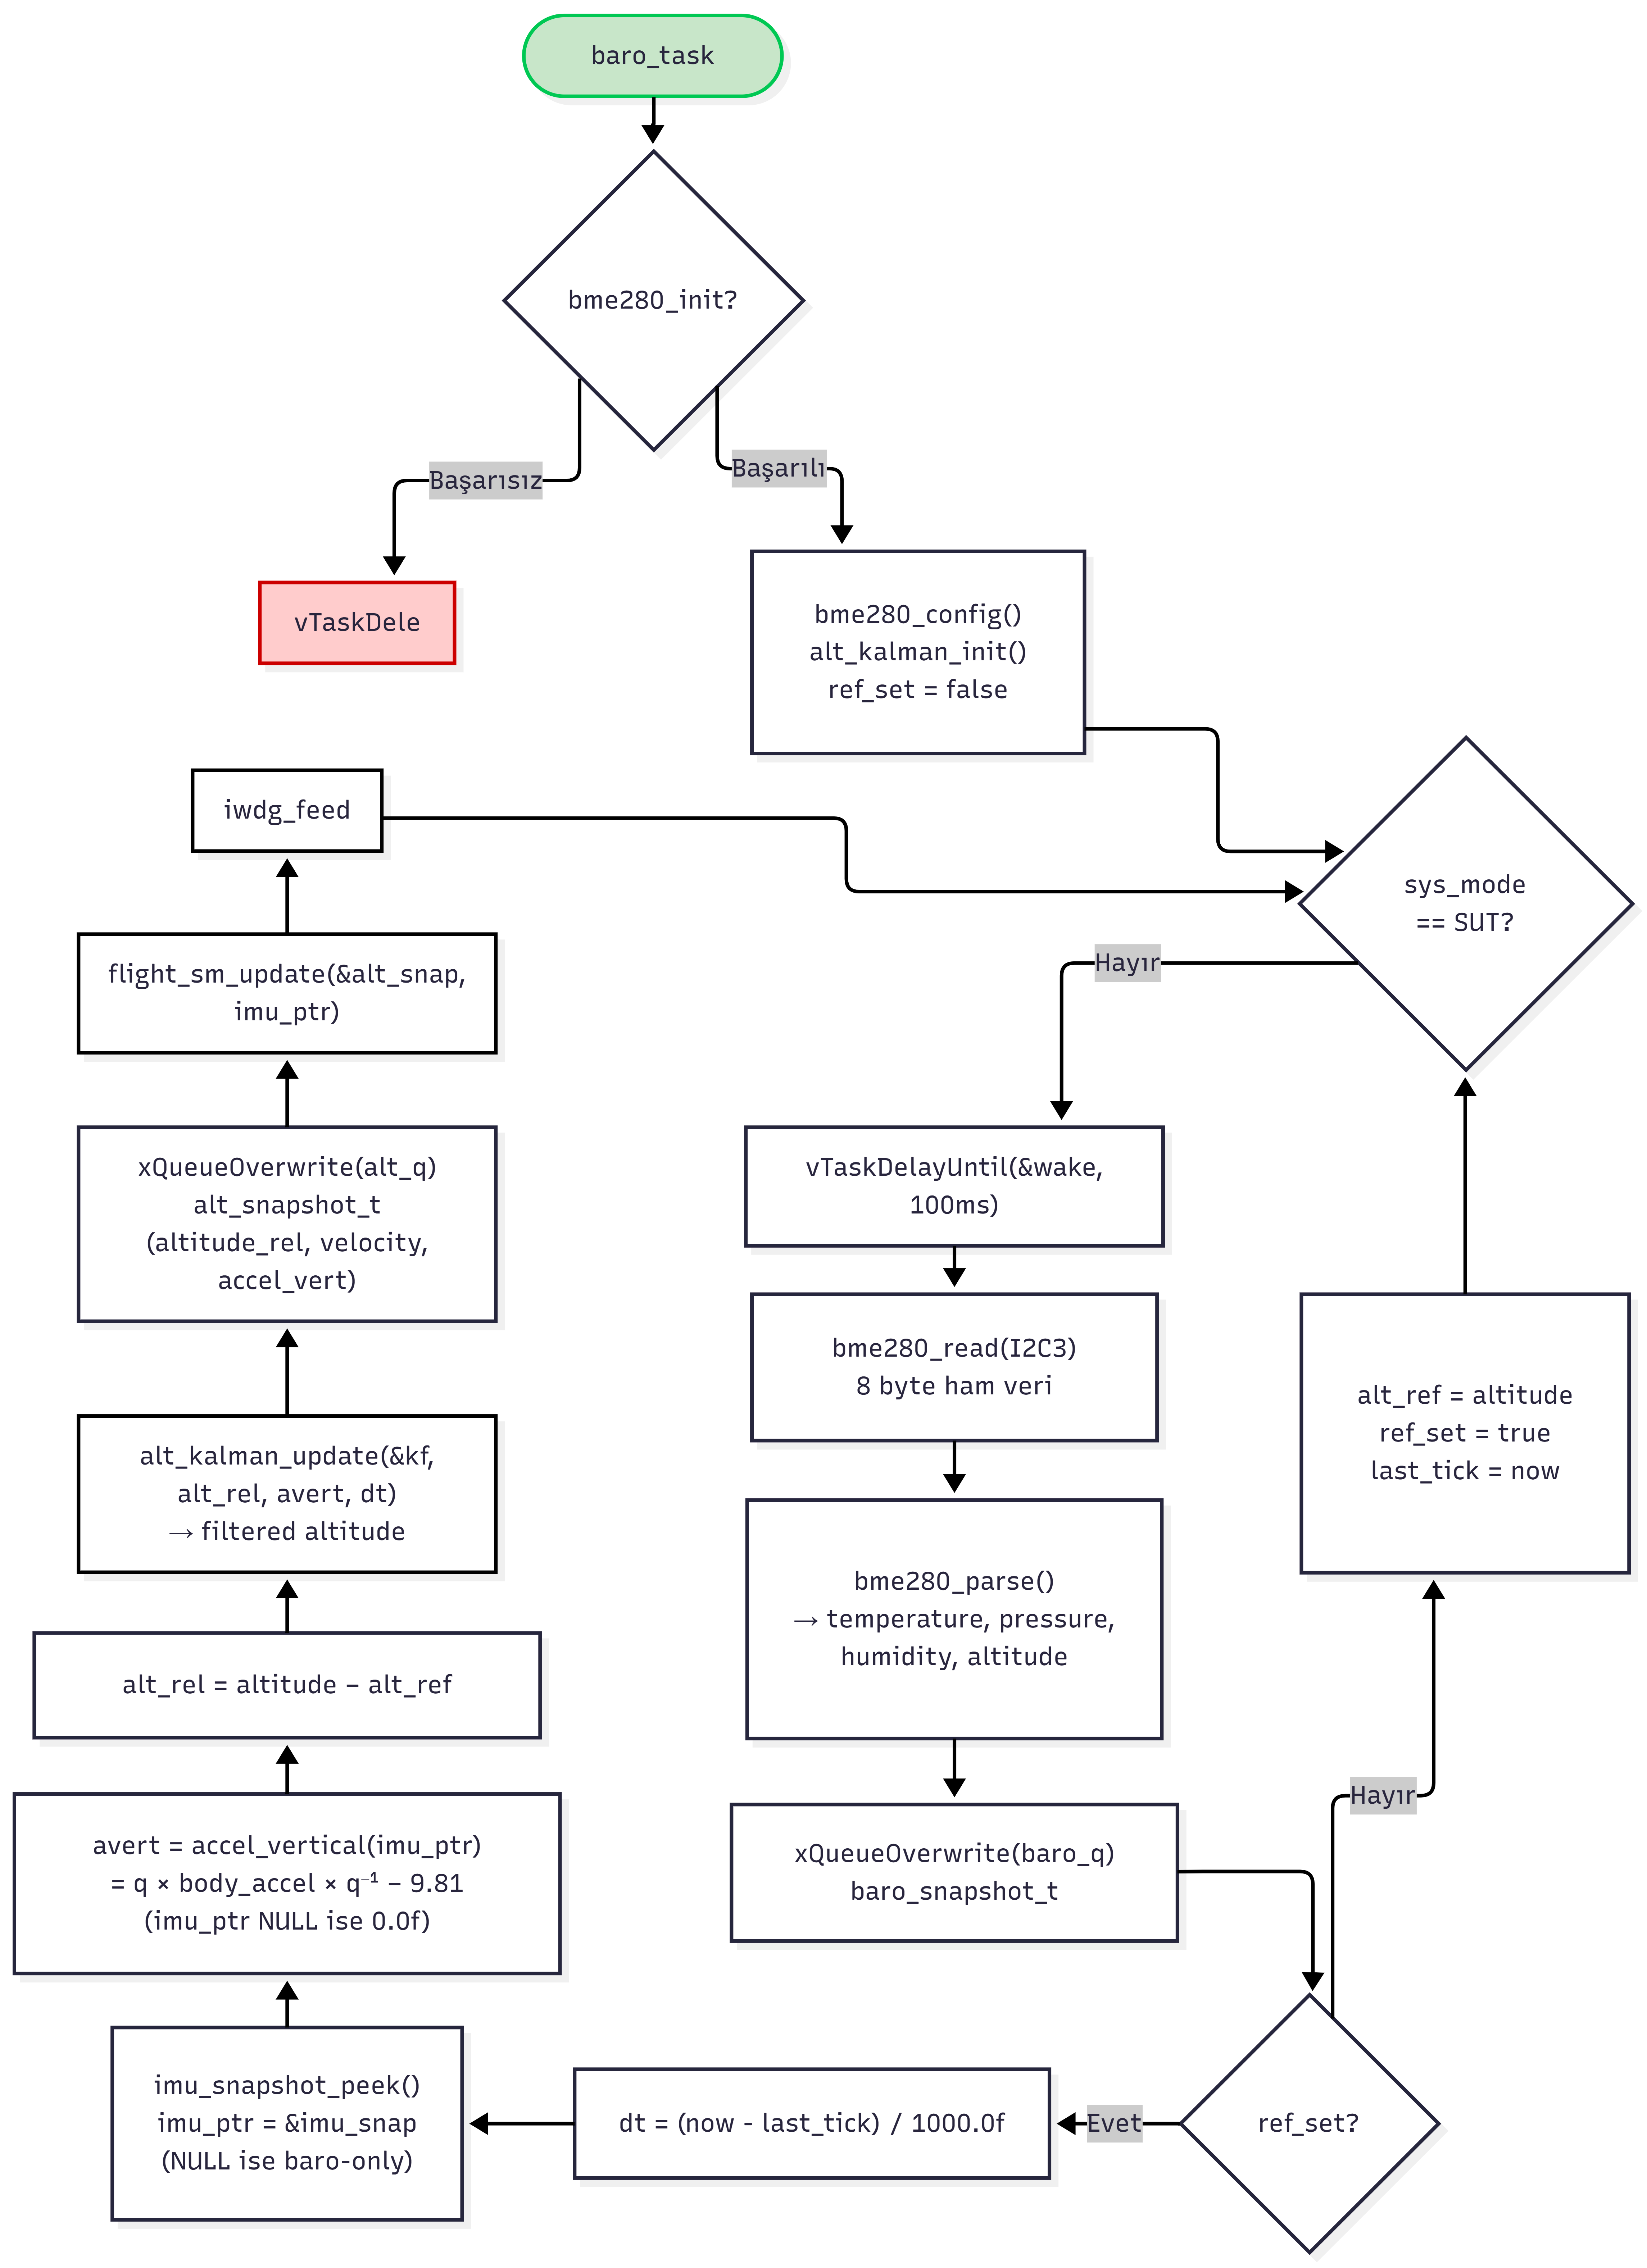
\includegraphics[width=\textwidth]{sekiller/Baro TaskAnaDöngüsü_veKalman_entegrasyonu.png}
    \caption{Barometre Ana Döngüsü, Kalman Filtresi ve FSM Entegrasyonu}
    \label{fig:baro_pipeline}
\end{figure}

\begin{lstlisting}[language=C, caption={10 Hz Barometre Okuma, Kalman ve Uçuş FSM Akışı (\texttt{baro\_task.c})}]
uint8_t raw[8];
if (bme280_read(&hi2c3, raw) != HAL_OK) continue;

bme280_parse(raw, &calib, &data);

float alt_rel  = data.altitude - alt_ref;
float filtered = alt_kalman_update(&kf, alt_rel, avert, dt);

flight_sm_update(&alt_snap, imu_ptr);
\end{lstlisting}

\subsubsection{L86 GNSS Modülü (Circular DMA, NMEA)}
Konum verisi, işlemci müdahalesi olmaksızın arabelleklerin kesintisiz dolmasını sağlayan Circular (Dairesel) DMA RX modeli kullanılarak USART6 üzerinden işlenmektedir. \verb|GNSS_BUF_HALF| arabelleğinin alt ve üst seviyesi dolduğunda ayrı yarı-kesmeler oluşturularak (\verb|0x01U|, \verb|0x02U|) NMEA katarı (\verb|GNRMC|, \verb|GPGGA|) \verb|sscanf| ile incelenip enlem, boylam, hız ve HDOP gibi argümanlar parçalanmaktadır.
Sistem başlarken L86 standart baud hızı olan 9600 bps seviyesinden \verb|$PMTK251| komutuyla 57600 bps geçişine ayarlanır. Veriler saniyede 1 kere (1 Hz) snapshot dosyasına yüklenir. Eğer GNSS sinyali uydulardan fix bulamazsa \verb|is_valid| bayrağı kapalı tutularak karar mekanizmalarının yanıltılması engellenmektedir.

\subsection{Sensör Füzyonu ve Durum Kestirimi}
\label{sensor_fuzyonu_ve_durum_kestirimi}

\subsubsection{Mahony AHRS Filtresi (6DOF Quaternion)}
Model roketin 3 boyutlu uzayda Euler açısı problemlerini (Gimbal Lock) devreden çıkarmak amacıyla hesaplama süreçlerinde \textit{Quaternion} formülasyonu kullanılmıştır. Mahony filtresinin öncelikli adımı normalize edilmiş ivme ile quaternion destekli tahmini yerçekiminin hatalarını çıkarıp ($\mathbf{e} = \hat{\mathbf{g}} \times \mathbf{a}_{norm}$) PI denetleyicisi ile sisteme dahil etmektir. 

Verimli işlem performansı için Quake III "Fast Inverse Square Root" (\verb|inv_sqrt|) kullanılarak ağırlık hafifletilmiştir. Kod içerisinde oransal kazanç ($K_p=2.0$) ve integral kazancı ($K_i=0.005$) olarak ele alınmıştır. Çıkan 6 eksen quaternion hesabı sırasıyla roll, pitch, yaw ve \textit{theta (eğim açısı)} verilerine dönüştürülür.

\begin{lstlisting}[language=C, caption={Mahony Quaternion Türevi Güncellemesi (\texttt{mahony.c})}]
/* Jiroskop hata duzeltmesi ve quaternion turevi */
float gx_corr = gx + m->twoKp * ex + m->integral[0];
float gy_corr = gy + m->twoKp * ey + m->integral[1];
float gz_corr = gz + m->twoKp * ez + m->integral[2];

float qDot1 = 0.5f * (-q2 * gx_corr - q3 * gy_corr - q4 * gz_corr);
float qDot2 = 0.5f * ( q1 * gx_corr + q3 * gz_corr - q4 * gy_corr);
/* ... diger quaternion carpimlari ve entegrasyon */
\end{lstlisting}

\subsubsection{Yükseklik Kalman Filtresi (Baro + IMU)}
Barometre ve IMU'dan elde edilen birbirinden farklı zemin karakteristiğine sahip iki veriyi optimum düzeyde birleştirmek için 3 boyutlu durum vektörüne sahip ($x = [\text{irtifa}, \text{hız}, \text{ivme\_bias}]^T$) geliştirilmiş yükseklik Kalman filtresi uyarlanmıştır. Filtrenin sistem geçiş ($F$), ölçüm modeli ($H$) ile zamanın karesel artış parametreleri ($Q$) tanımlanmıştır:

\begin{equation}
F = \begin{bmatrix}
1 & \Delta t & \Delta t^2/2 \\
0 & 1 & \Delta t \\
0 & 0 & 1
\end{bmatrix} \quad , \quad
H = \begin{bmatrix}
1 & 0 & 0 \\
0 & 0 & 1
\end{bmatrix} \quad , \quad
Q = q \begin{bmatrix}
\frac{\Delta t^4}{4} & \frac{\Delta t^3}{2} & \frac{\Delta t^2}{2} \\
\frac{\Delta t^3}{2} & \Delta t^2 & \Delta t \\
\frac{\Delta t^2}{2} & \Delta t & 1
\end{bmatrix}
\end{equation}

\begin{figure}[H]
    \centering
    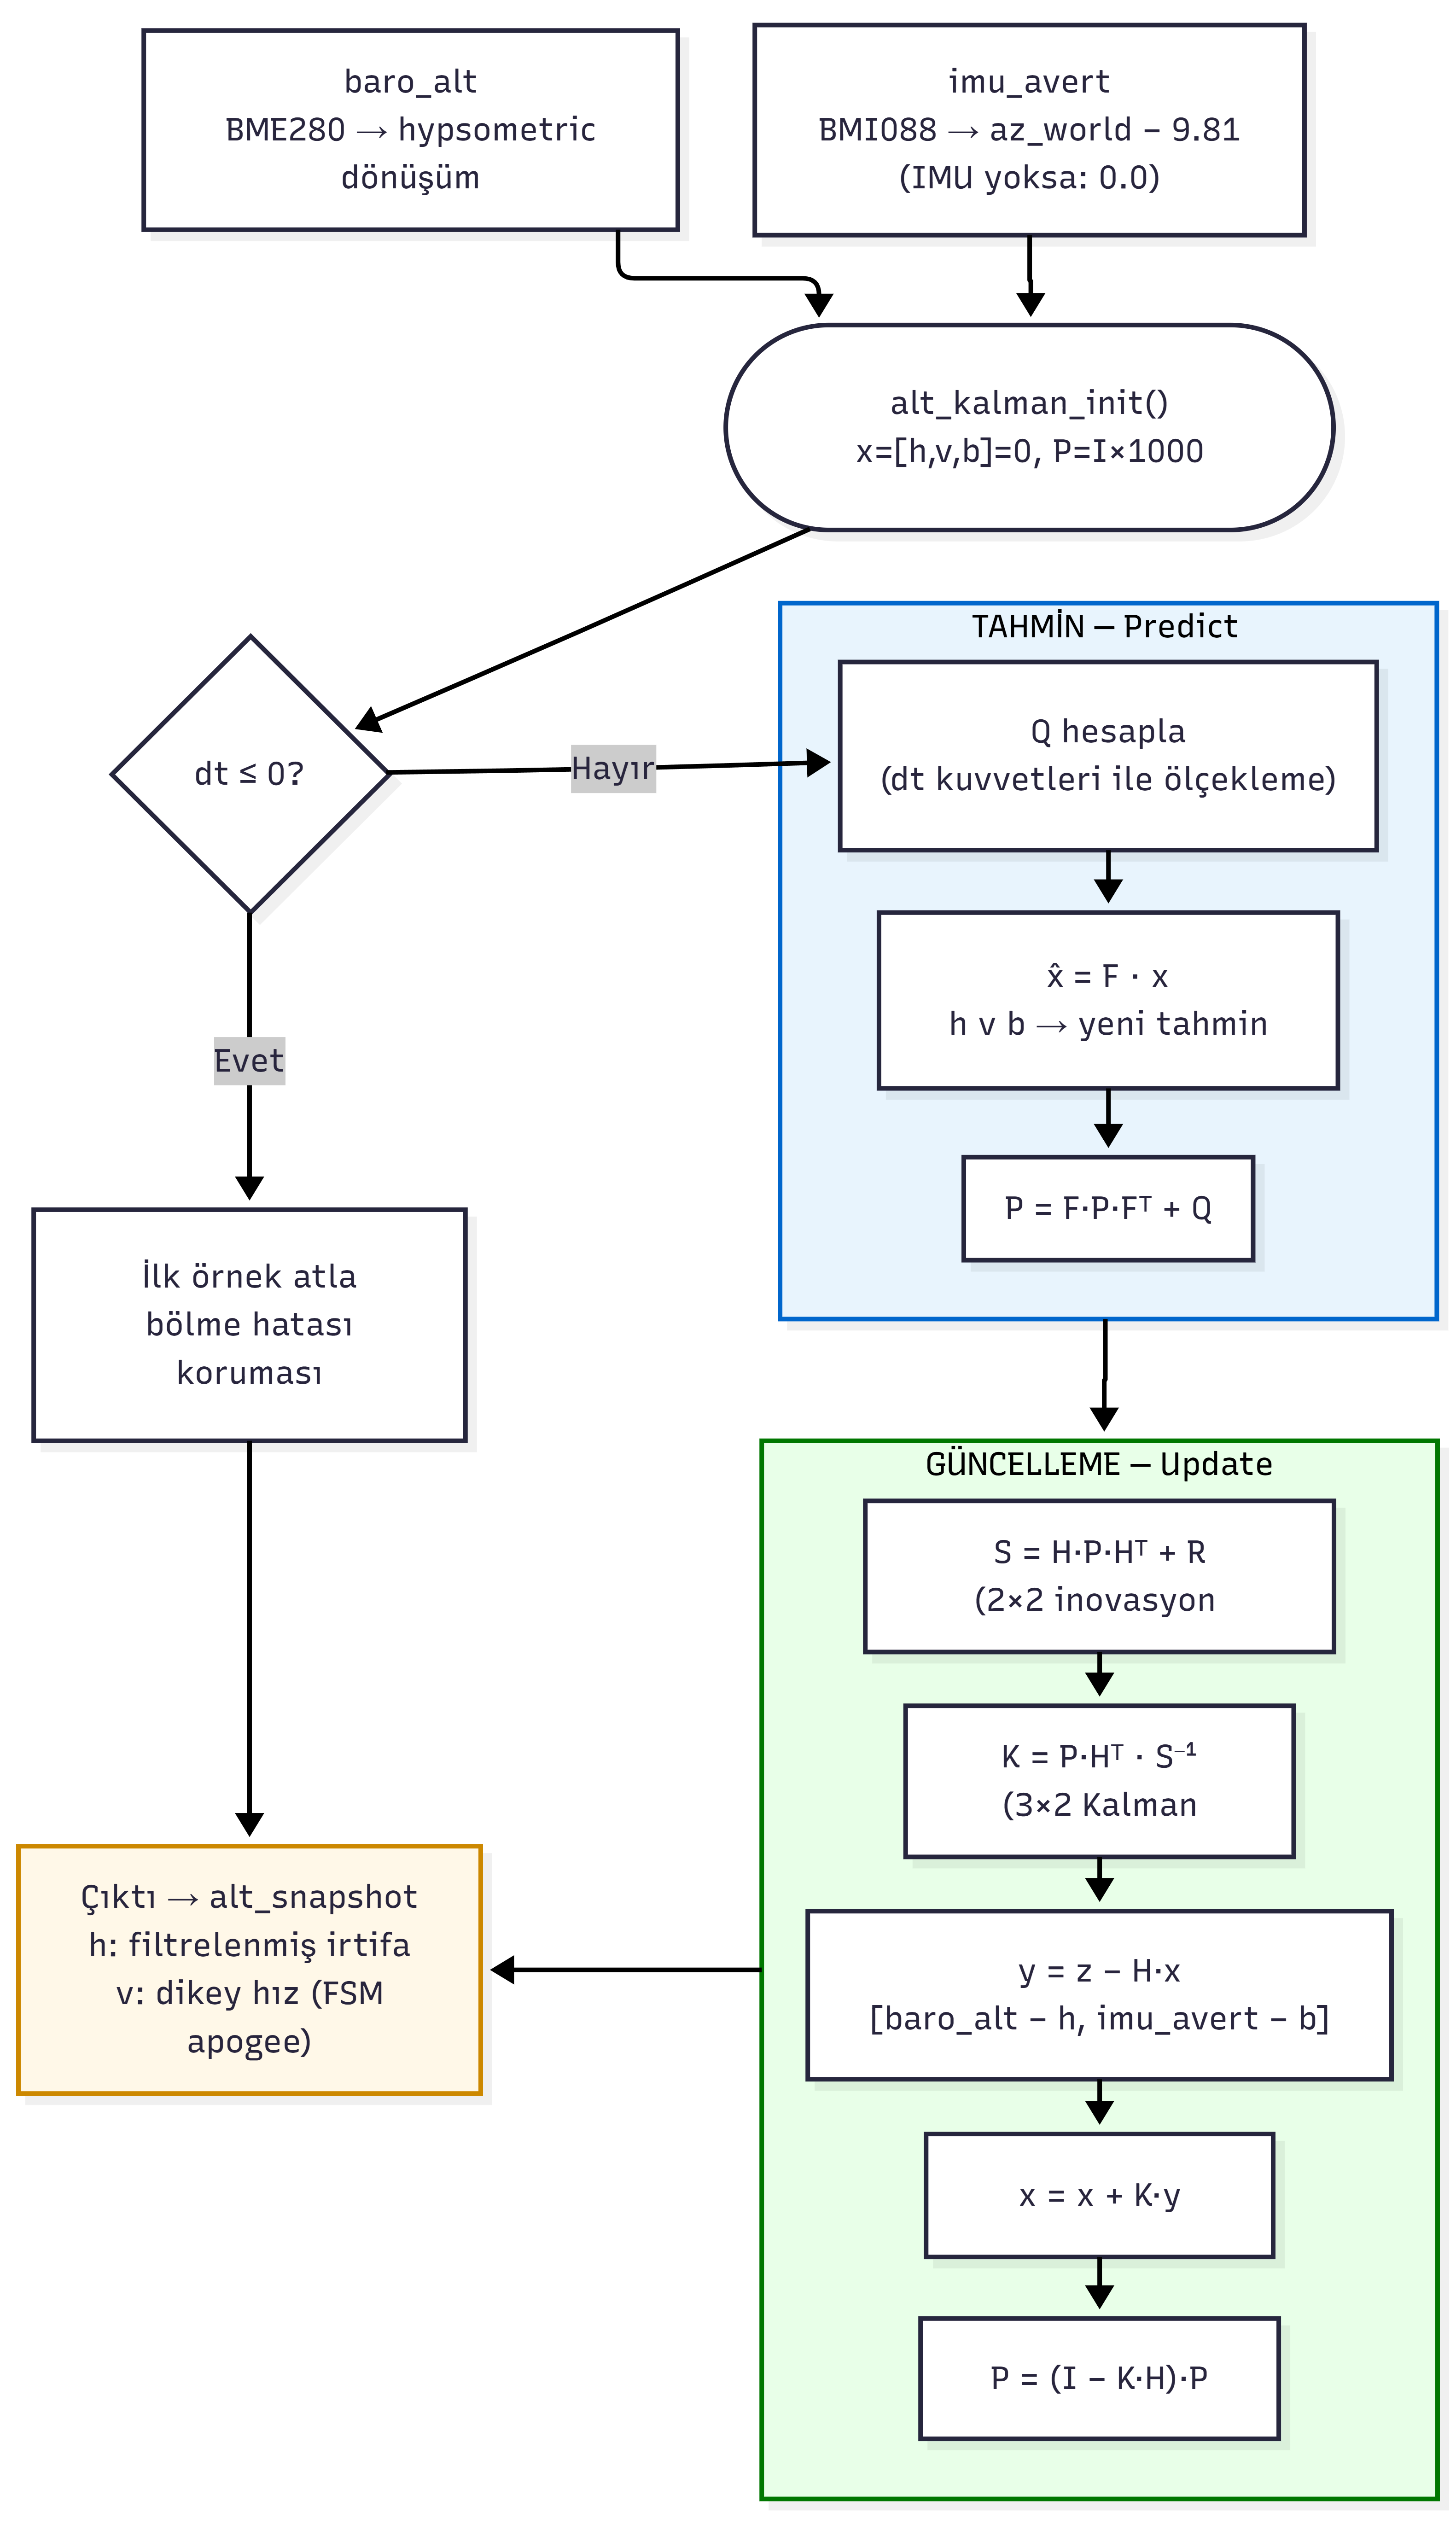
\includegraphics[width=\textwidth]{sekiller/KalmanFiltresi.png}
    \caption{3-Durumlu Baro-IMU Yükseklik Kalman Filtresi Döngüsü}
    \label{fig:kalman_filter}
\end{figure}

Filtrede ayarlanan ($r\_alt = 5.0$, bari gürültüsü) ve ($r\_acc = 10.0$ ivme gürültüsü) gibi varyanslar, filtrenin hangi sensöre daha çok güveneceği ayarını (tuning mantığını) temsil etmektedir. İlk kalkış adımında bölü sıfır hatasının yaşanmaması için \verb|dt <= 0.0f| koruması koda eklenerek kazanç ($K$) oluşturulmuş, son adımda durum matrisleri irtifa ve ivme kullanılarak matris-çarpım tersi ile ($2 \times 2$) güncellenmiştir.

\subsection{Uçuş Durum Makinesi (7 Faz FSM)}
\label{ucus_durum_makinesi}

Model roketin fırlatılışından kurtarma mekanizmalarının ayrılmasına kadarki süreç karmaşık bir Durum Makinesi (Finite State Machine) modülünde ele alınır. 

\begin{itemize}
    \item \textbf{IDLE'dan BOOST'a Geçiş:} Sensörden alınan IMU fırlatma ivmesinin $> 45 m/s^2$ (veya IMU hatasında barometrenin $> 15 m/s$ hız) yakalaması sonucu tetiklenir.
    \item \textbf{BOOST'dan COAST'a Geçiş:} Kalman filtresinin dikey ivmesinin aralıksız 5 örnek ($500 ms$) boyunca $0$'ın altına düşmesi ya da acil durum $8$ sn zaman aşımının oluşmasıyla motordaki yanmanın bittiğine karar verilir. (Burnout).
    \item \textbf{COAST'dan APOGEE'ye Geçiş:} Kalman dikey hızı 0'ın altında kaldığında veya \textit{Tilt (Eğim)} durumu 70 derecenin üzerine çıktığında tespit edilir. Roket apogee (tepe noktasında) olduğunu anladığı anda ilk fırlatma (Drogue) GPIO'su tetiklenir. Çift güvenlik sensörüyle (hem hız, hem açı) tetikleme sağlanır.
    \item \textbf{MAIN DESCENT ve LANDED Geçişi:} İrtifa $300 m$'nin altına indiğinde barometre tetikleyici oluşturur, yere iniş hızı saniyeler (< 2 m/s) ile kesinleştirilip uçuş işlemi sonlandırılır.
\end{itemize}

\begin{figure}[H]
    \centering
    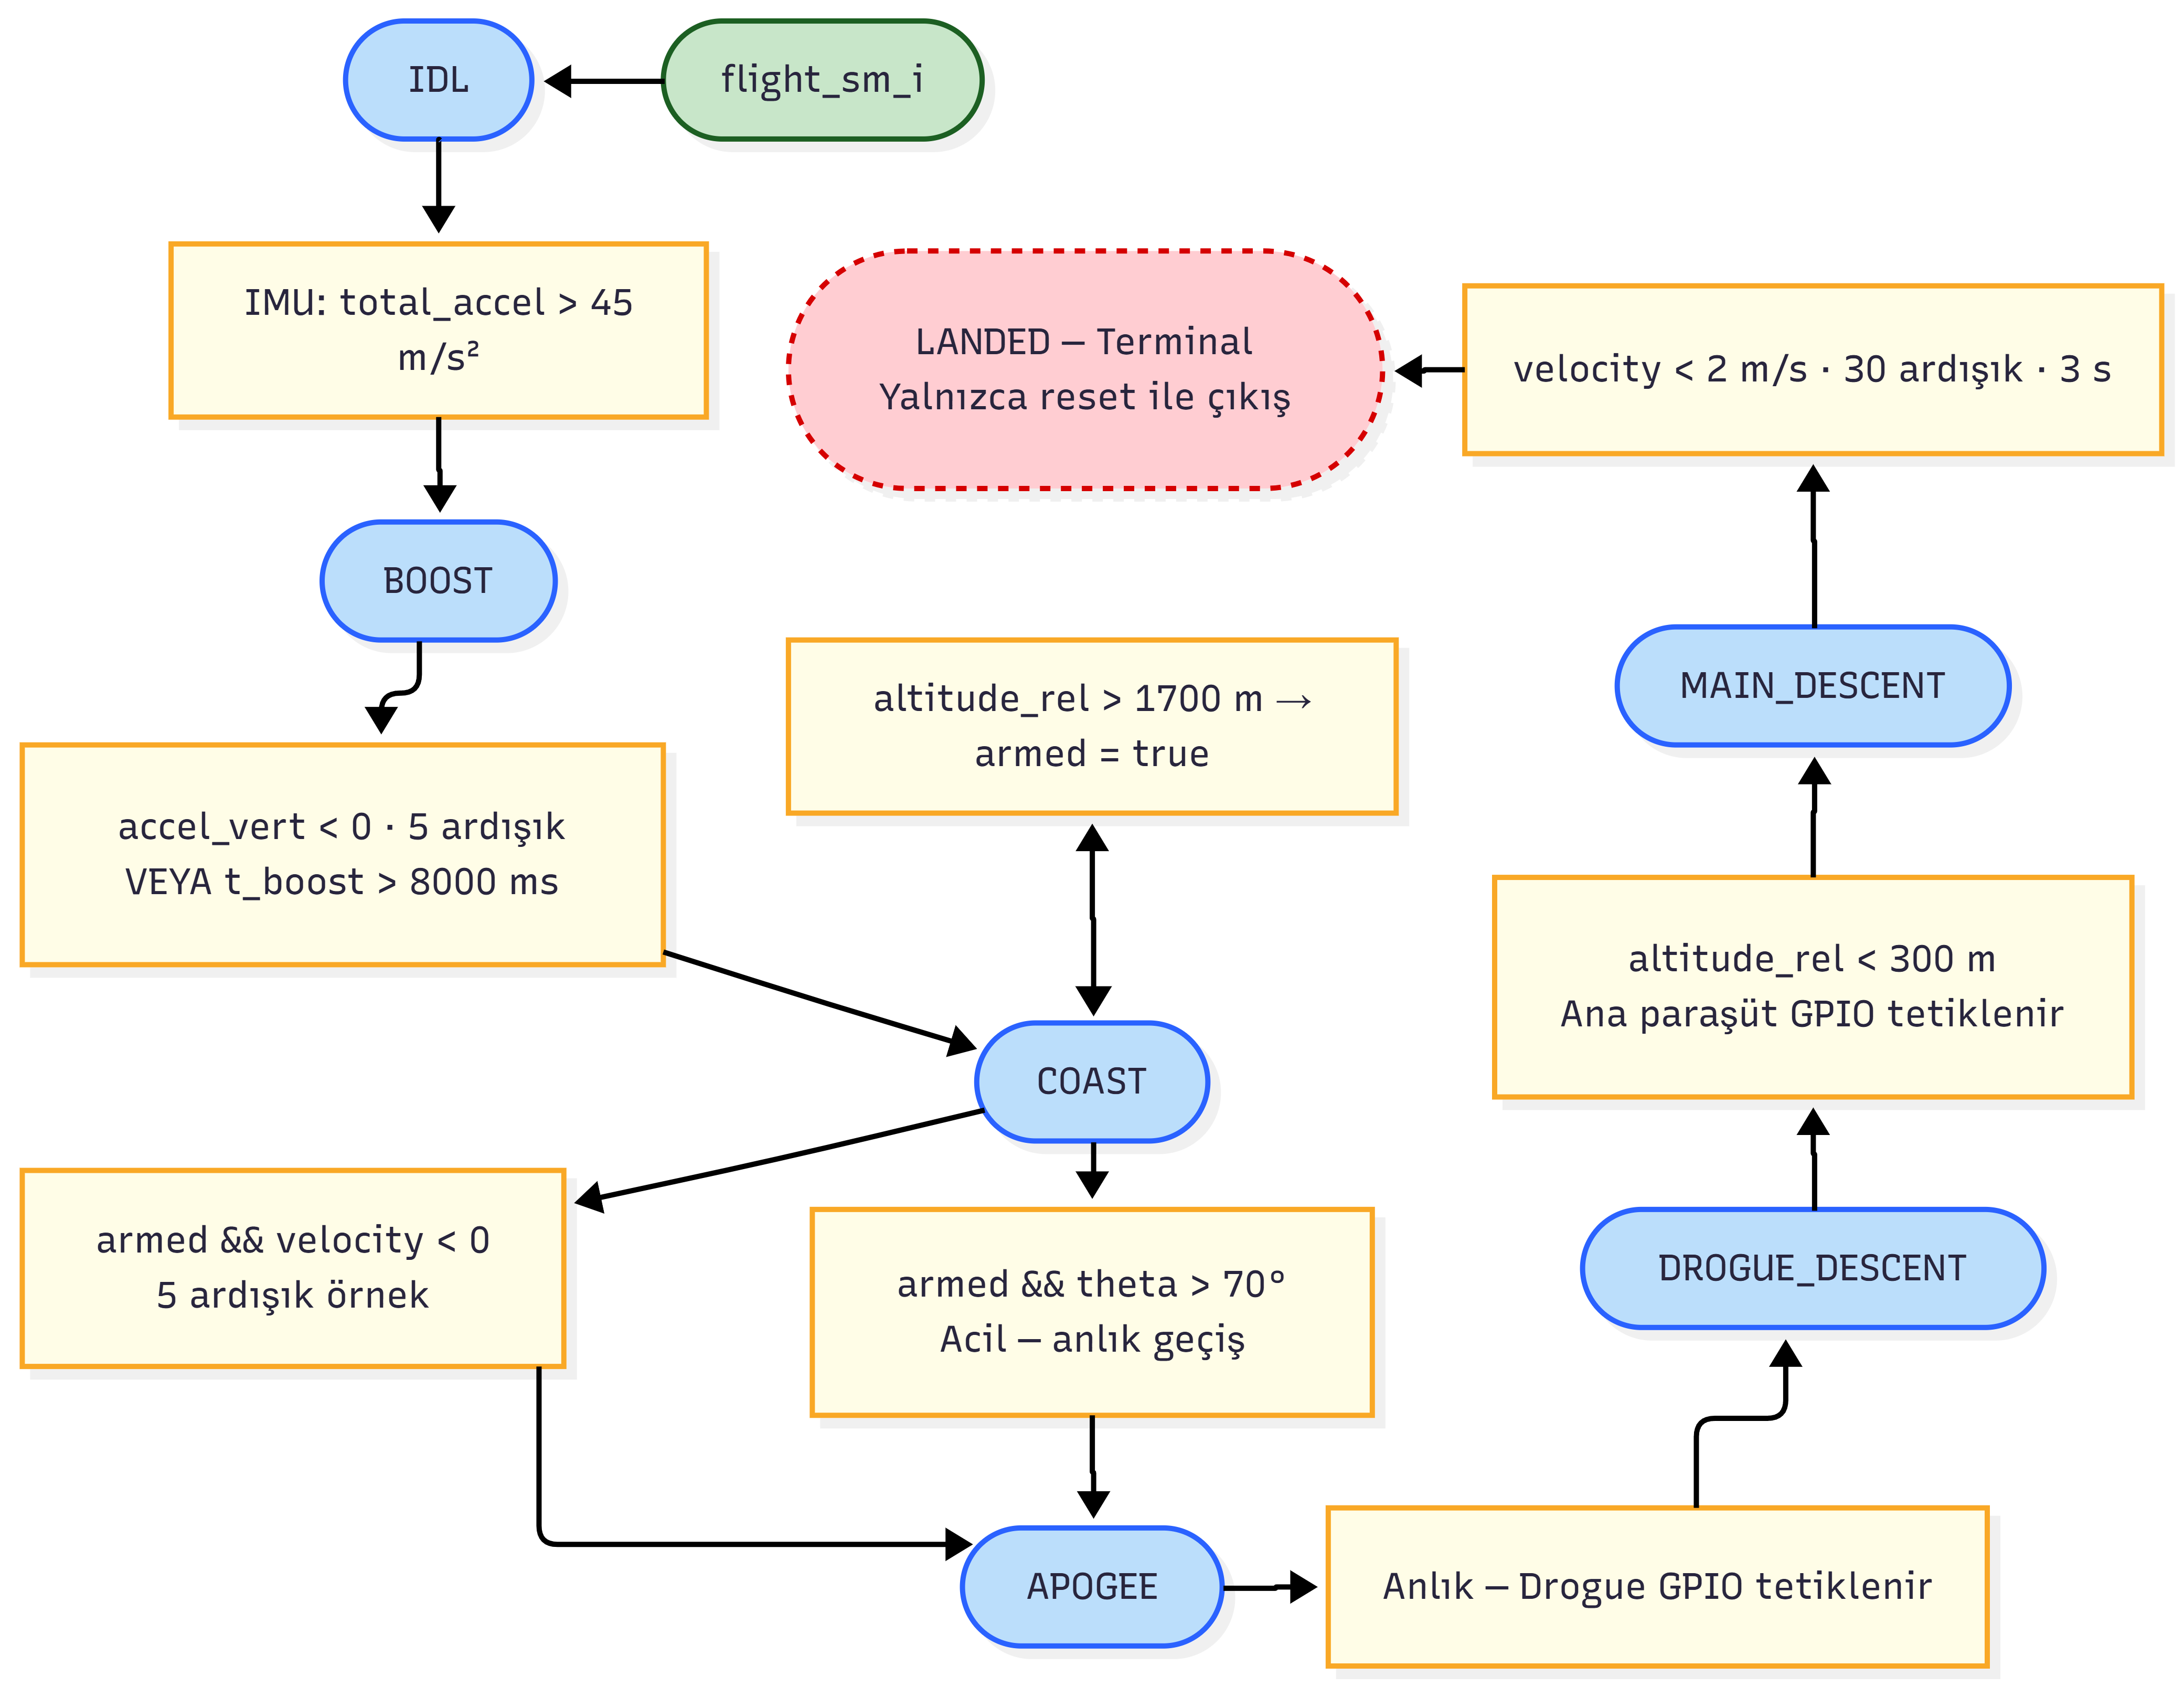
\includegraphics[width=\textwidth]{sekiller/UçuşDurumMakinesi.png}
    \caption{Uçuş Durum Makinesi (FSM) 7-Faz Durum Geçiş Mekanizması}
    \label{fig:ucus_fsm}
\end{figure}

\subsection{Güvenilirlik Mekanizmaları}
\label{guvenilirlik_mekanizmalari}

Dış etmen veya döngü bloklamasından oluşabilecek hayati aviyonik arızalarına karşı aşağıdaki yazılımsal ve donanımsal korumalar entegre edilmiştir.

\subsubsection{IWDG Watchdog ve Yığın Aşım (Stack Overflow) Koruması}
Sistemdeki donanımsal Watchdog $2$ saniyelik zaman aşımına (\textit{timeout}) sahiptir. Barometre görevi (\verb|baro_task|) 100 ms aralıklarla \verb|iwdg_feed()| beslemesi yapar. Eğer görev donarsa, sistem doğrudan kendini sonlandırıp baştan uyanarak sensör veri kurtarmasına gider.
Ayrıca, görevlerin RAM içerisinde kendisine verilenden fazla bir boyutu talep etmesi (Stack Overflow) durumu, sistem başlarken aktive edilen \verb|configCHECK_FOR_STACK_OVERFLOW| ile FreeRTOS kancası (hook) tarafından durdurulup yeniden başlatılmaktadır.

\subsubsection{IMU Başarısızlığında Baro-Only (Kısıtlandırılmış/Degraded) Mod}
Başlangıç durumunda veya kalkıştan sonra \verb|bmi_init| iletişim döngüsünün tam anlamıyla tahrip olması sistemin tamamen kaybolmasına neden teşkil etmez. Sistem böyle bir tabloda; roket fırlatıldı durumunu (BOOST tahmini), sadece hızlanarak kalkan Kalman baro hızı ile sağlar $> 15 m/s$. Ancak tilt-bazlı apogee pasifize edilip, tepe noktasında yedek güvenlik kamerasız çalışır. 

\subsection{Test ve Doğrulama Metodolojisi}
\label{test_ve_dogrulama_metodolojisi}

Model roketin kritik uçuş dinamiklerini simüle edebilmek ve uçuş bilgisayarı algoritmalarını yer istasyonunda test edebilmek amacıyla çeşitli sistem test modülleri (SIT ve SUT) entegre edilmiştir. Bu modüller donanım ile bilgisayar (Python arayüzü) arasındaki köprüyü oluşturmaktadır.

\subsubsection{SIT — Sensör İzleme Testi}
Bu metodoloji, sensör verilerinin doğrudan mikrodenetleyiciden okunarak bir bilgisayar ortamına (Python GUI) yansıtılıp canlı incelenmesini hedefler. Algoritmaların doğru çalışıp çalışmadığını değil; STM32 ve sensörler arasındaki donanımsal sürücü iletişim yollarını (DMA, I2C, USART2 transferleri) doğrulamak amaçlanmıştır. 

Statik ortam testinde IMU çıktılarının (Z ekseni yaklaşık -9.81 $m/s^2$ yerçekimi ivmesi olacak haliyle) doğruluğu, barometrik irtifanın bulunulan konum koşullarıyla uyuşmazlığı hesaplanarak Mahony denklemlerinden roll, pitch, yaw gibi veriler de 3 boyutlu roket dönüşüm modelinde görselleştirilir.

\begin{figure}[H]
    \centering
    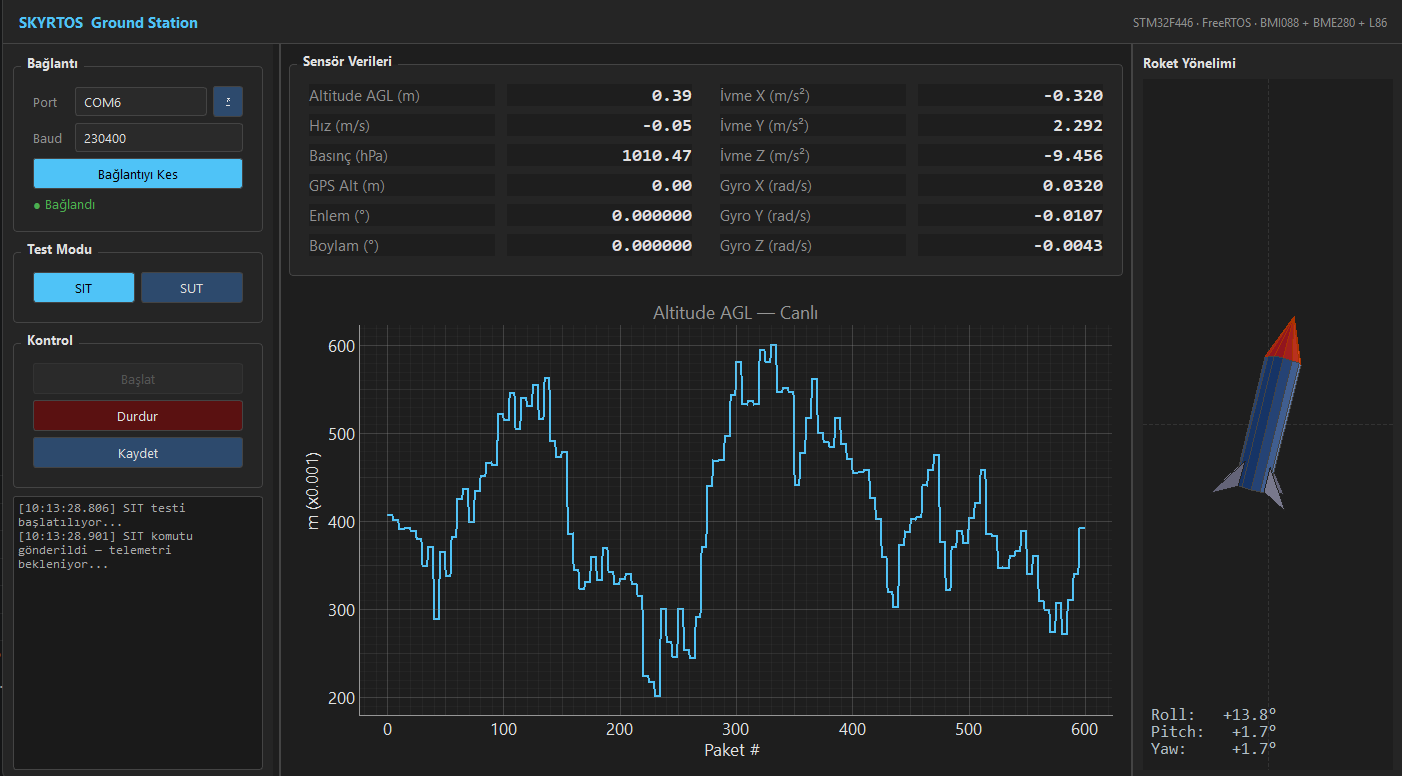
\includegraphics[width=\textwidth]{sekiller/SIT_testi_arayüz.png}
    \caption{Python GUI Canlı Sensör İzleme ve Yönelim 3D Görselleştirmesi (SIT)}
    \label{fig:sit_test}
\end{figure}

\begin{table}[H]
    \centering
    \caption{SIT Test Senaryoları ve Beklenen Yanıtlar}
    \label{tab:sit_senaryolar}
    \begin{tabular}{|p{4cm}|p{6cm}|p{5cm}|}
    \hline
    \textbf{Test Olayı} & \textbf{Beklenen Tepki} & \textbf{Test Durumu} \\ \hline
    Masaüstü Statik Test & Z İvmesi: $-9.81 m/s^2$, X ve Y: $\sim 0$ & Kalibrasyon ve referans uyumu sağlandı. \\ \hline
    Euler ve Quaternion İzleme & XYZ Ekseninde 3 Boyutlu Dönüşler & Gimbal Lock açmazı engellendi, yansıması başarılı. \\ \hline
    Baro Referans Doğrulaması & 0 Metre Rölatif (Göreli) İrtifa Set Edilmeli & Çevresel stabilite, ofset sıfırlandı. \\ \hline
    \end{tabular}
\end{table}

\subsubsection{SUT — Sentetik Uçuş Testi (Processor-in-the-Loop)}
SUT metodolojisinde ("Processor-in-the-Loop"), algoritma tepkilerini ve 7-faz FSM kararlarını test etmek maksadıyla RocketPy \cite{rocketpy} açık kaynak simülatöründen faydalanılmıştır. Bu test modunda, PC simüle edilmiş ivme ve irtifa okumalarını UART üzerinden peyderpey STM32 uçuş bilgisayarına yollar. 

Bu süreçte STM32'de yeralan \verb|imu_task|, \verb|baro_task|, \verb|telemetry_task| ve \verb|gnss_task| modülleri \verb|MODE_SUT| kontrolüne takılarak \verb|portMAX_DELAY| ile uyutulur; CPU simüle edilmiş \verb|sut_task| tarafından harcanır. Sistem, PC den aldığı verileri Mahony ve Kalman filtrelerinden geçirir ve Python platformuna Cevap Paketi (SUT\_RESPONSE) olarak aynen iletir.

SUT Haberleşme yapısında kullanılan temel cevap paketi formatı alt kısımda tablolanmıştır (STM32 den PC'ye):
\begin{table}[H]
    \centering
    \caption{SUT Response UART Paketi İçeriği (Toplam 26 Bayt)}
    \label{tab:sut_response}
    \begin{tabular}{|l|l|l|l|}
    \hline
    \textbf{Offset} & \textbf{Bayt / Veri Tipi} & \textbf{Paket İçeriği} \\ \hline
    0 & 1 (uint8\_t) & Başlangıç Header (0xAE) \\ \hline
    1 - 4 & 4 (float) & Simülasyon Zamanı (sim\_time) \\ \hline
    5 - 8 & 4 (float) & Filtrelenmiş İrtifa Verisi \\ \hline
    9 - 20 & 12 (3 x float) & Roll, Pitch ve Yaw Deg Açıları \\ \hline
    21 - 22 & 2 (uint16\_t) & FSM Durumu (HIGH/LOW Byte) \\ \hline
    23 & 1 (uint8\_t) & Sağlama Toplamı (Checksum) \\ \hline
    24 - 25 & 2 & Bitiş (0x0D, 0x0A - CR LF) \\ \hline
    \end{tabular}
\end{table}

\begin{figure}[H]
    \centering
    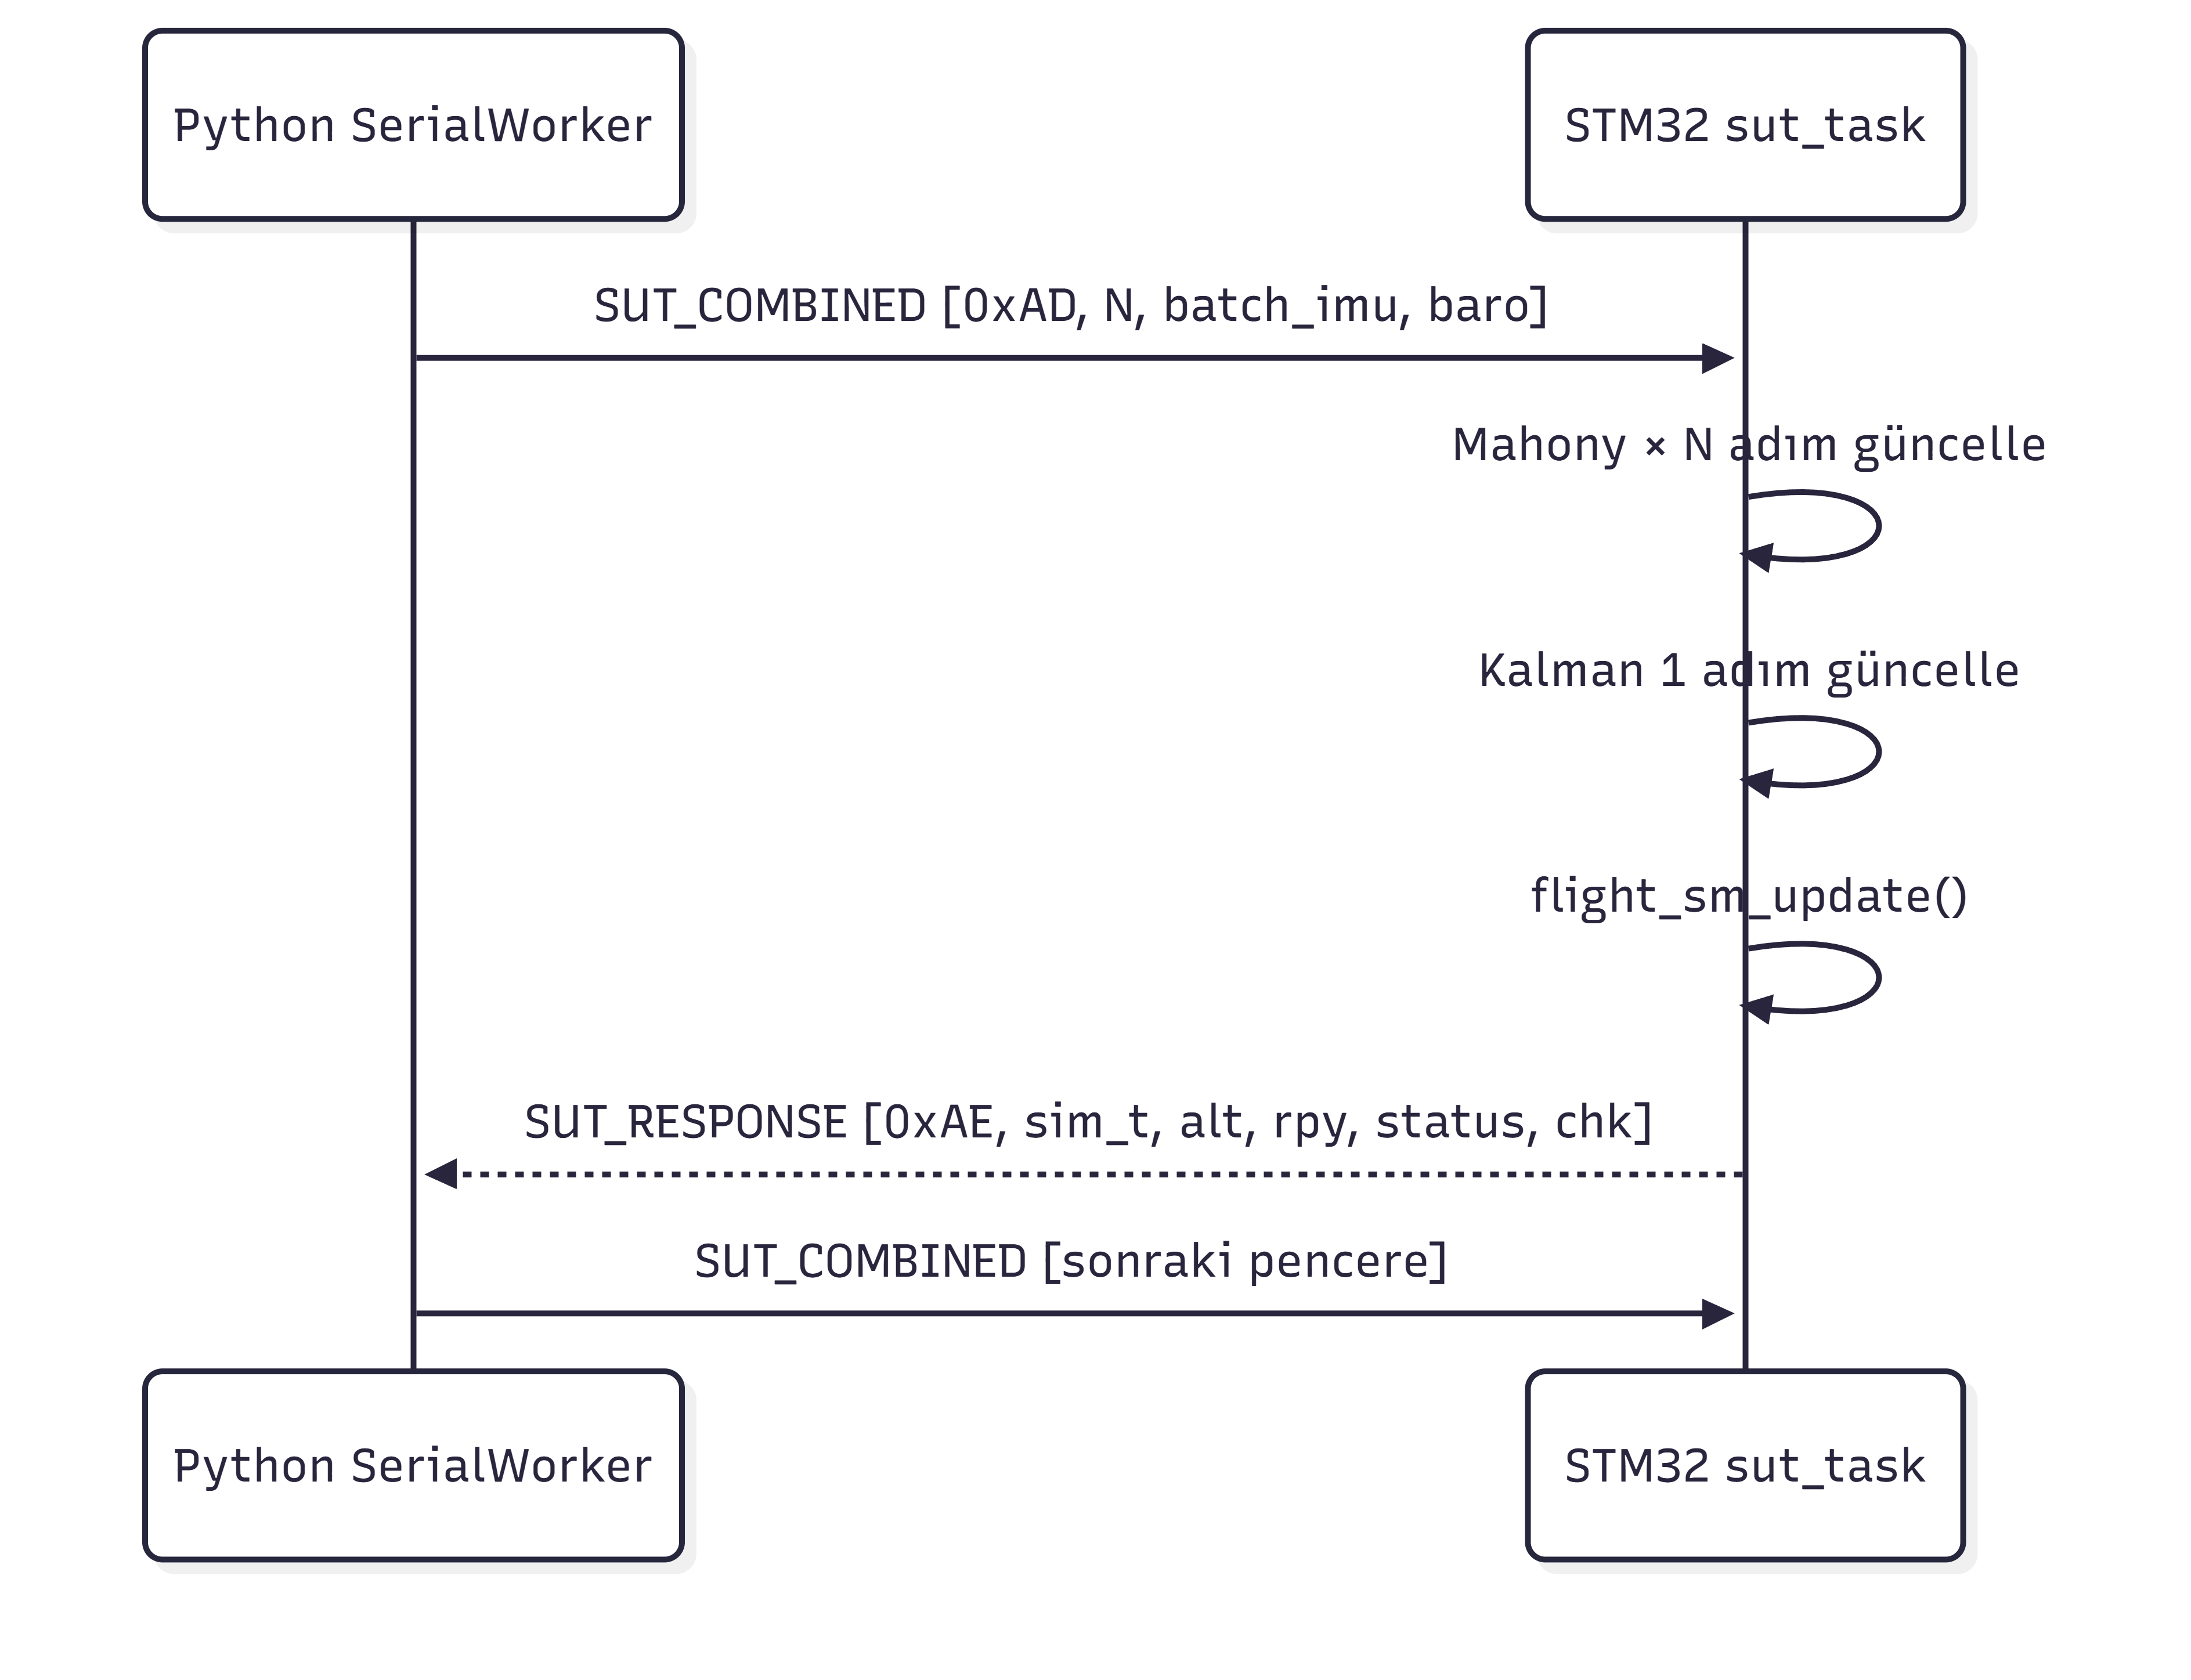
\includegraphics[width=0.8\textwidth]{sekiller/SUT_SistemMimarisi.png}
    \caption{Processor-in-the-Loop Veri Aktarım Akışı (SUT)}
    \label{fig:sut_mimarisi}
\end{figure}

Aşağıdaki pseudo-code (sözde kod), STM32 \verb|sut_task| dairesel veri analiz mimarisini yansıtmaktadır:
\begin{lstlisting}[language=C, caption={SUT İşleyişi Pseudo-Code Özeti}]
// cmd_task ile iletilen bildirimler
if (sut_queue_receive(&pkt)) {
    for (int i = 0; i < pkt.imu_count; i++) {
        // Gyro-only (Mahony Batch hesaplamalari)
        mahony_update(&mah, pkt.imu[i].gx ... dt); 
    }
    float filtered = alt_kalman_update(&kf, alt_rel, 0.0f, dt_baro);
    flight_sm_update(&alt_snap, &imu_snap);
    sut_send_response(..., filtered, roll, pitch, yaw, flight_status);
}
\end{lstlisting}

\subsubsection{RocketPy Simülasyon Verisi ve Test Altyapısı}
Simülatöre girdi olarak \textbf{RocketPy} ortamı kullanılmış ve aviyonik karta sentetik olarak yollanacak sanal atmosferik ile statik veriş akışı CSV tablolarına kaydedilmiştir. Sisteme entegre edilen Python parametreleri gereksinimlerin testine olanak tanır:

\begin{figure}[H]
    \centering
    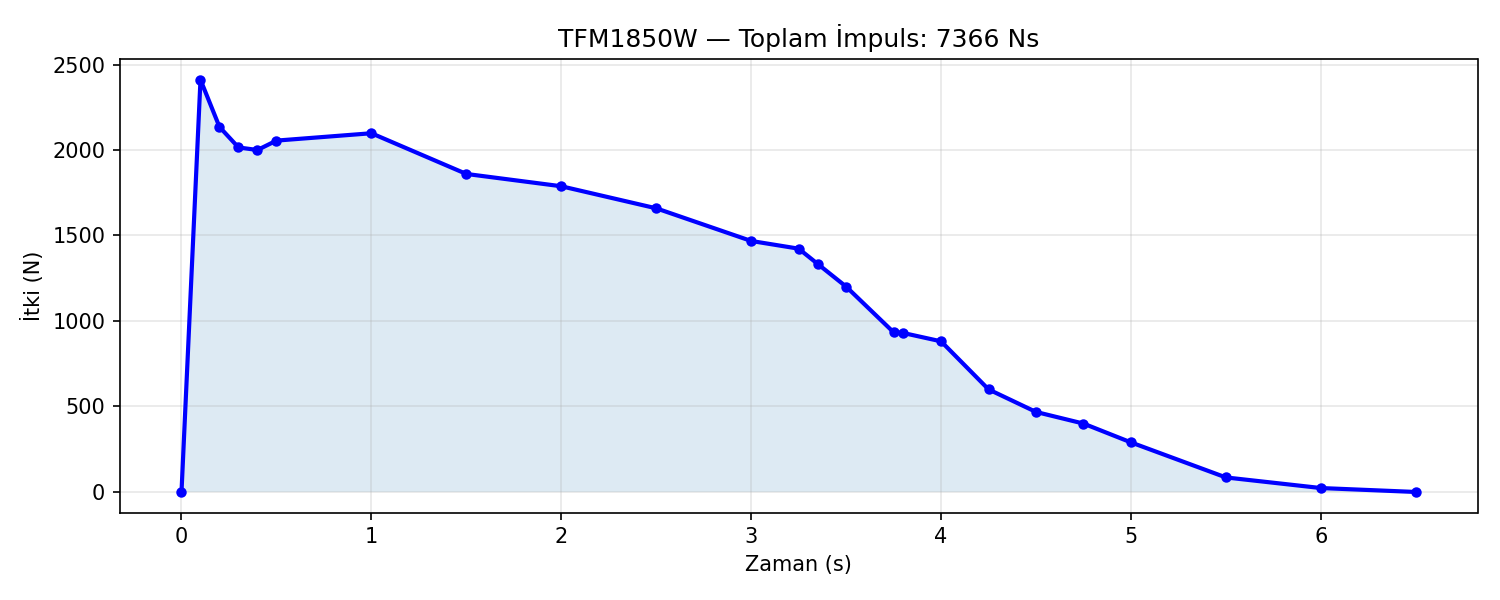
\includegraphics[width=0.8\textwidth]{sekiller/motor_thrust.png}
    \caption{RocketPy Simülasyonunda Kullanılan Motor İtme Kuvveti (Thrust) Eğrisi}
    \label{fig:motor_thrust}
\end{figure}

\begin{lstlisting}[language=Python, caption={RocketPy Motor, Roket Boyutları ve Atmosfer Ortamı Tanımlamaları}]
from rocketpy import SolidMotor, Rocket, Environment

motor = SolidMotor(
    thrust_source="data/TFM1850W.eng",  # Itme egrisi
    dry_mass=6.693,                     # Kuru kutle (kg)
    burn_time=6.5,                      # Yanma suresi (s)
    # diger degiskenler ...
)

rocket = Rocket(
    radius=0.056,                       # Govde yaricapi (56 mm)
    mass=15.166,                        # Motorsuz kuru kutle
    power_off_drag=0.45,                
    power_on_drag=0.45,
    center_of_mass_without_motor=1.13,  # CG, kuyruktan (m)
)
rocket.add_motor(motor, position=0.0)

env = Environment(
    latitude=39.90, longitude=32.80, elevation=900.0  # Ankara referansi
)
env.set_atmospheric_model(type="standard_atmosphere")
\end{lstlisting}

Simülasyon sonucunda elde edilen teorik irtifa ve ivme grafikleri sensörlerin SUT modu üzerinden test edilmesi için temel referans modelleri olarak CSV dosyalarına kaydedilmektedir.

\begin{figure}[H]
    \centering
    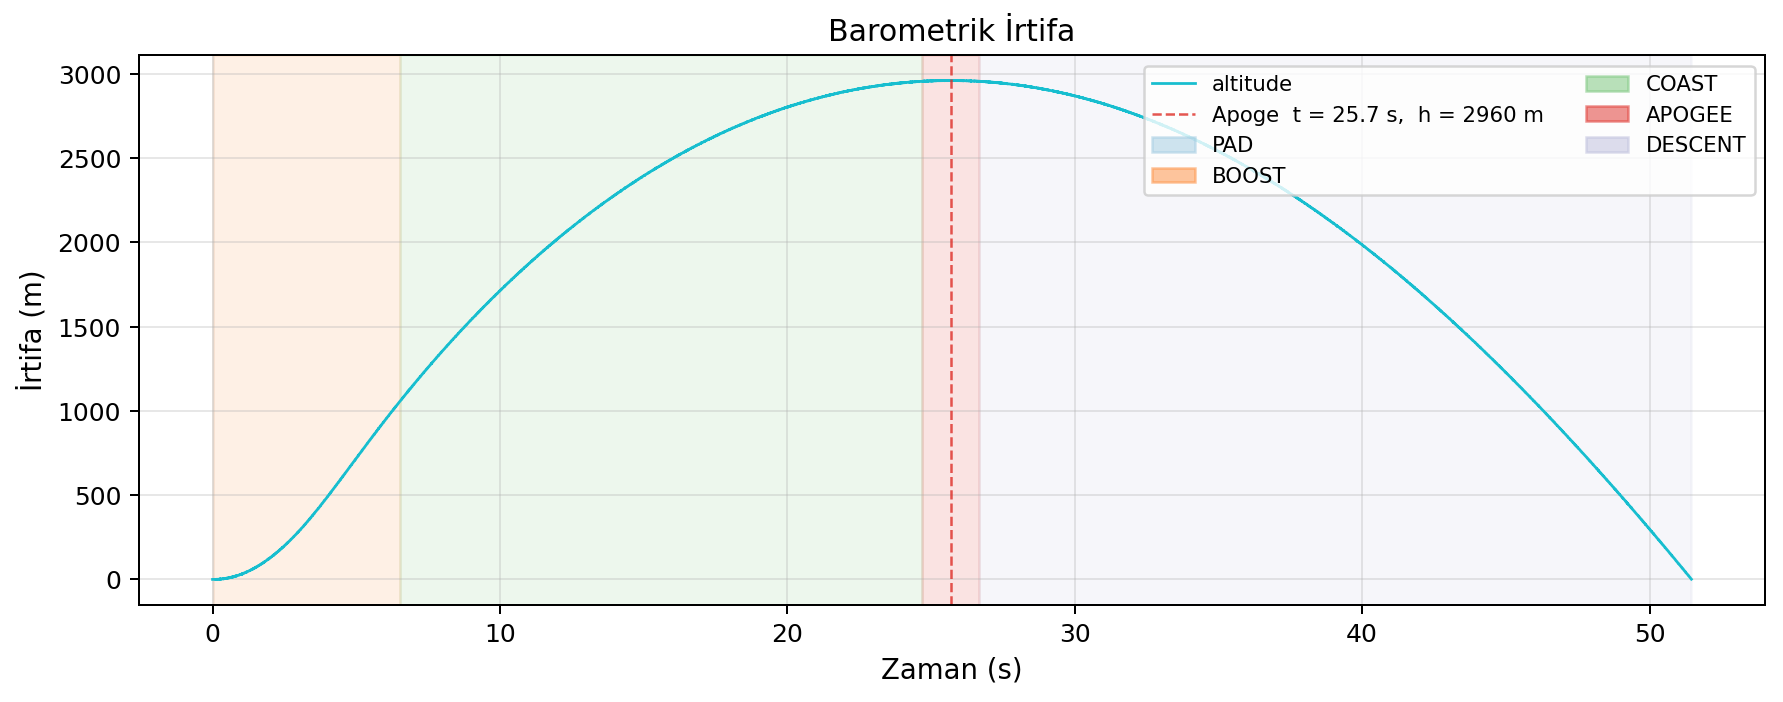
\includegraphics[width=0.8\textwidth]{sekiller/fig_altitude.png}
    \caption{RocketPy Simülasyonu Teorik İrtifa-Zaman Grafiği}
    \label{fig:rocketpy_altitude}
\end{figure}

\begin{figure}[H]
    \centering
    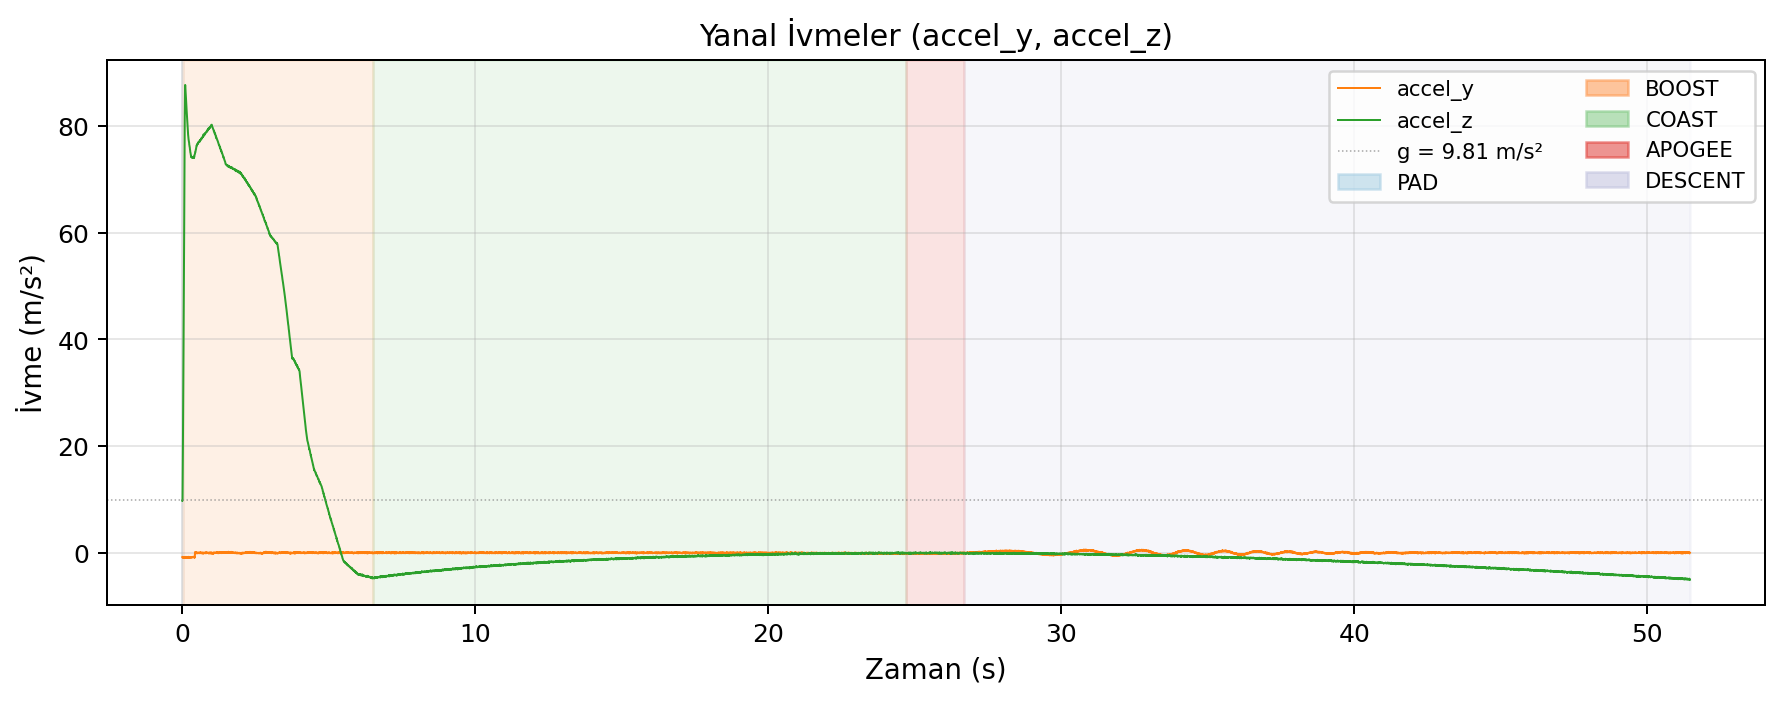
\includegraphics[width=0.8\textwidth]{sekiller/fig_accel_yz.png}
    \caption{RocketPy Simülasyonu Teorik İvme (Y-Z Ekseni) Grafiği}
    \label{fig:rocketpy_accel}
\end{figure}

Algoritmalar bu sistem üzerinde koşturulduktan sonra STM32 tarafından "PyQtGraph" ekranına (Hız, zaman, İvme vb.) durum çizgisi basılarak uçuş evresi analiz edilmektedir.

\clearpage